\RequirePackage[l2tabu,orthodox]{nag}

% TODO: decide if one-sided/two-sided
%\documentclass[headsepline,footsepline,footinclude=false,fontsize=11pt,paper=a4,listof=totoc,bibliography=totoc,BCOR=12mm,DIV=12]{scrbook} % two-sided
\documentclass[headsepline,footsepline,footinclude=false,oneside,fontsize=11pt,paper=a4,listof=totoc,bibliography=totoc]{scrbook} % one-sided

\PassOptionsToPackage{table,svgnames,dvipsnames}{xcolor}

\usepackage[utf8]{inputenc}
\usepackage[T1]{fontenc}
\usepackage[sc]{mathpazo}
\usepackage[american]{babel}
\usepackage[autostyle]{csquotes}
\usepackage[%
  backend=biber,
  url=false,
  style=alphabetic,
  maxnames=4,
  minnames=3,
  maxbibnames=99,
  firstinits,
  uniquename=init]{biblatex} % TODO: adapt bibliography style
\usepackage{graphicx}
\usepackage{scrhack} % necessary for listings package
\usepackage{listings}
\usepackage{lstautogobble}
\usepackage{tikz}
\usepackage{pgfplots}
\usepackage{pgfplotstable}
\usepackage{booktabs}
\usepackage[final]{microtype}
\usepackage{caption}
\usepackage[hidelinks]{hyperref} % hidelinks removes colored boxes around references and links
\usepackage[toc,nonumberlist,acronym]{glossaries} % TODO: remove if glossary not needed

\bibliography{bibliography/literature}

\setkomafont{disposition}{\normalfont\bfseries} % use serif font for headings
\linespread{1.05} % adjust line spread for mathpazo font

% Settings for glossaries TODO: remove the following block if glossary not needed
\renewcommand{\glsnamefont}[1]{\normalfont\bfseries #1} % use serif font for glossary entry titles
\makeglossaries{}

% Settings for pgfplots
\pgfplotsset{compat=1.9} % TODO: adjust to your installed version
\pgfplotsset{
  % For available color names, see http://www.latextemplates.com/svgnames-colors
  cycle list={CornflowerBlue\\Dandelion\\ForestGreen\\BrickRed\\},
}

% Settings for lstlistings
\lstset{%
  basicstyle=\ttfamily,
  columns=fullflexible,
  autogobble,
  keywordstyle=\bfseries\color{MediumBlue},
  stringstyle=\color{DarkGreen}
}

% Basic information for cover & title page
\newcommand*{\getUniversity}{Technische Universität München}
\newcommand*{\getFaculty}{Department of Informatics}
\newcommand*{\getTitle}{TODO: Thesis title}
\newcommand*{\getTitleGer}{TODO: Titel der Abschlussarbeit}
\newcommand*{\getAuthor}{TODO: Author}
\newcommand*{\getDoctype}{TODO: Thesis type (Bachelor's Thesis in Informatics, Master's Thesis in Robotics, \ldots)}
\newcommand*{\getSupervisor}{TODO: Supervisor}
\newcommand*{\getAdvisor}{TODO: Advisor}
\newcommand*{\getSubmissionDate}{TODO: Submission date}
\newcommand*{\getSubmissionLocation}{Munich}

% TODO: add custom commands etc.


% TODO: remove if glossary not needed
\newglossaryentry{computer}
{
  name=computer,
  description={is a machine that\ldots}
}

\newacronym{tum}{TUM}{Technische Universität München}


\newcolumntype{R}[1]{>{\raggedleft\let\newline\\\arraybackslash\hspace{0pt}}m{#1}}

\begin{document}

\begin{titlepage}
  % HACK for two-sided documents: ignore binding correction for cover page.
  % Adapted from Markus Kohm's KOMA-Script titlepage=firstiscover handling.
  % See http://mirrors.ctan.org/macros/latex/contrib/koma-script/scrkernel-title.dtx,
  % \maketitle macro.
  \oddsidemargin=\evensidemargin\relax
  \textwidth=\dimexpr\paperwidth-2\evensidemargin-2in\relax
  \hsize=\textwidth\relax

  \centering

  
\includegraphics[width=40mm]{logos/tum}

  \vspace{5mm}
  {\huge\MakeUppercase{\getFaculty{}}}\\

  \vspace{5mm}
  {\large\MakeUppercase{\getUniversity{}}}\\

  \vspace{20mm}
  {\Large Secure Coding Phase 2}
  %{\Large \getDoctype{}}

  \vspace{15mm}
  %{\huge\bfseries \getTitle{}}

  \vspace{15mm}
  {\LARGE Team 3:
  	 Patrick Sattler, Aurel Roci, Stefan Kohler}
  %{\LARGE \getAuthor{}}

  \vspace{20mm}
  
\includegraphics[width=20mm]{logos/faculty}
\end{titlepage}


\frontmatter{}


{
	\chapter{Executive Summary}\

   \textbf{Secode21}\\

	We found several vulnerabilities, which could cause severe damage to the \textit{Secode21}. It is possible to get access to the admin page via stealing the session. Thus an attacker can register an arbitrary employee or customer and unlock the registered user. An	attacker can also execute a brute force attack on known user ids as there is no lock mechanism to prevent this. Besides the security issues there is also a severe problem with regard to the business logic. In the current state this web application should not be used productively!	\\


	\textbf{Team3 Online Banking}\\

	We found some issues, which potentially could cause damage to the \textit{Team3 Online Banking}. However the detected issues are quite easy to fix. If an experienced attacker performs a man in the middle attack he'll be able to track session ids. The implications are severe, as the	attacker can take over the role of the customer, but this attack requires advanced knowledge. With regard to the business logic there was only one issue with low risk detected. \\

	\textbf{Comparison}\\

	In summary we were able to clearly state out that the \textit{Team3 Online Banking} web application has less and also less severe vulnerabilites then the \textit{Secode21} web application. Furthermore it has to be said that the detected issues of the \textit{Team3 Online Banking} are easier to fix and will cost less money to implement.
}

\pagebreak
%\begin{titlepage}
  \centering

  
\includegraphics[width=40mm]{logos/tum}

  \vspace{5mm}
  {\huge\MakeUppercase{\getFaculty{}}}\\

  \vspace{5mm}
  {\large\MakeUppercase{\getUniversity{}}}\\
 
  \vspace{20mm}
  {\Large \getDoctype{}}

  \vspace{15mm}
  {\huge\bfseries \getTitle{}}

%  \vspace{10mm}
%  {\huge\bfseries \getTitleGer{}}

  \vspace{15mm}
%  \begin{tabular}{l l}
%    Author: & \getAuthor{} \\
%    Supervisor: & \getSupervisor{} \\
%    Advisor: & \getAdvisor{} \\
%    Submission Date: & \getSubmissionDate{} \\
%  \end{tabular}

  \vspace{20mm}
  
\includegraphics[width=20mm]{logos/faculty}
\end{titlepage}

%\thispagestyle{empty}
\vspace*{0.8\textheight}
\noindent
I confirm that this \MakeLowercase{\getDoctype{}} is my own work and I have documented all sources and material used.

\vspace{15mm}
\noindent
\getSubmissionLocation{}, \getSubmissionDate{} \hspace{5cm} \getAuthor{}

\cleardoublepage{}

%\addcontentsline{toc}{chapter}{Acknowledgments}
\thispagestyle{empty}

\vspace*{2cm}

\begin{center}
{\usekomafont{section} Acknowledgments}
\end{center}

\vspace{1cm}

%TODO: Acknowledgments

\cleardoublepage{}

%\chapter{\abstractname}

%TODO: Abstract



\microtypesetup{protrusion=false}
\tableofcontents{}
\microtypesetup{protrusion=true}

\mainmatter{}

\chapter{Time Tracking Table}
%\chapter{Introduction}\label{chapter:introduction}

\section{Section}
Citation test~\parencite{latex}.

\subsection{Subsection}
See~\autoref{fig:sample}.

\begin{figure}[htpb]
  \centering
  
\includegraphics{logos/tum}
  \caption[Example figure]{An example for a figure.}\label{fig:sample}
\end{figure}

\section{Section}

See~\autoref{tab:sample}, \autoref{fig:sample-drawing}, \autoref{fig:sample-plot}, \autoref{fig:sample-listing}.

\begin{table}[htpb]
  \caption[Example table]{An example for a simple table.}\label{tab:sample}
  \centering
  \begin{tabular}{l l l l}
    \toprule
      A & B & C & D \\
    \midrule
      1 & 2 & 1 & 2 \\
      2 & 3 & 2 & 3 \\
    \bottomrule
  \end{tabular}
\end{table}

\begin{figure}[htpb]
  \centering
  % This should probably go into a file in figures/
  \begin{tikzpicture}[node distance=3cm]
    \node (R0) {$R_1$};
    \node (R1) [right of=R0] {$R_2$};
    \node (R2) [below of=R1] {$R_4$};
    \node (R3) [below of=R0] {$R_3$};
    \node (R4) [right of=R1] {$R_5$};

    \path[every node]
      (R0) edge (R1)
      (R0) edge (R3)
      (R3) edge (R2)
      (R2) edge (R1)
      (R1) edge (R4);
  \end{tikzpicture}
  \caption[Example drawing]{An example for a simple drawing.}\label{fig:sample-drawing}
\end{figure}

\begin{figure}[htpb]
  \centering

  \pgfplotstableset{col sep=&, row sep=\\}
  % This should probably go into a file in data/
  \pgfplotstableread{
    a & b    \\
    1 & 1000 \\
    2 & 1500 \\
    3 & 1600 \\
  }\exampleA
  \pgfplotstableread{
    a & b    \\
    1 & 1200 \\
    2 & 800 \\
    3 & 1400 \\
  }\exampleB
  % This should probably go into a file in figures/
  \begin{tikzpicture}
    \begin{axis}[
        ymin=0,
        legend style={legend pos=south east},
        grid,
        thick,
        ylabel=Y,
        xlabel=X
      ]
      \addplot table[x=a, y=b]{\exampleA};
      \addlegendentry{Example A};
      \addplot table[x=a, y=b]{\exampleB};
      \addlegendentry{Example B};
    \end{axis}
  \end{tikzpicture}
  \caption[Example plot]{An example for a simple plot.}\label{fig:sample-plot}
\end{figure}

\begin{figure}[htpb]
  \centering
  \begin{tabular}{c}
  \begin{lstlisting}[language=SQL]
    SELECT * FROM tbl WHERE tbl.str = "str"
  \end{lstlisting}
  \end{tabular}
  \caption[Example listing]{An example for a source code listing.}\label{fig:sample-listing}
\end{figure}

% TODO: add more chapters here
\chapter{Vulnerabilities Overview}
Based on our testing, we identified the following vulnerabilities for the Secode21
Bank and the OnlineBanking Bank:
\section{Secode21}
\subsection{Static Session ID} \
\begin{itemize}
	\item Likelihood: \textit{high}
	\item Implication: \textit{high}
	\item Risk: \textit{high}
	\item Reference: OWASP OTG-SESS-003
\end{itemize}

The session id is saved in form of the (static) user id in a cookie. This cookie can be used on any machine
to take over the account of a user. The lifetime of this cookie is only limited by the cookie lifetime field.


\subsection{Stored XSS in Registration} \
\begin{itemize}
	\item Likelihood: \textit{medium}
	\item Implication: \textit{high}
	\item Risk: \textit{high}
	\item Reference: OWASP OTG-INPVAL-002
\end{itemize}

Using stored cross-site-scripting attacks, one can inject JavaScript code, that is run, when the Administrator/Employee logs in. Arbitrary code can be loaded from a third party page.

\subsection{Brute Force Password} \
\begin{itemize}
	\item Likelihood: \textit{high}
	\item Implication: \textit{medium}
	\item Risk: \textit{medium}
	\item Reference: OWASP OTG-AUTHN-003
\end{itemize}
The application has no lock out mechanism, which allows brute force attacks on known usernames and testing
for a valid password


\subsection{Directory Traversal} \
\begin{itemize}
	\item Likelihood: \textit{high}
	\item Implication: \textit{medium}
	\item Risk: \textit{medium}
	\item Reference: OWASP OTG-AUTHN-001
\end{itemize}
The application has no lock out mechanism, which allows brute force attacks on known usernames and testing
for a valid password



\section{Team3 Online Banking}

\subsection{Static Session ID}\label{Static Session ID}\
\begin{itemize}
	\item Likelihood: \textit{high}
	\item Implication: \textit{high}
	\item Risk: \textit{high}
	\item Reference: OWASP OTG-SESS-003
\end{itemize}

The session id is saved in form of the (static) user id in a cookie. This cookie can be used on any machine
to take over the account of a user. The lifetime of this cookie is only limited by the cookie lifetime field.


\subsection{Stored XSS in Registration}\label{Stored XSS in Registration}\
\begin{itemize}
	\item Likelihood: \textit{medium}
	\item Implication: \textit{high}
	\item Risk: \textit{high}
	\item Reference: OWASP OTG-INPVAL-002
\end{itemize}

Using stored cross-site-scripting attacks, one can inject JavaScript code, that is run, when the Administrator/Employee logs in. Arbitrary code can be loaded from a third party page.

\subsection{{Brute Force Password}}\label{Missing Lock Out Mechanism}\
\begin{itemize}
	\item Likelihood: \textit{high}
	\item Implication: \textit{medium}
	\item Risk: \textit{medium}
	\item Reference: OWASP OTG-AUTHN-003
\end{itemize}
The application has no lock out mechanism, which allows brute force attacks on known usernames and testing
for a valid password


\section{Vulnerability Overview}

\chapter{Detailed Report}

The following pages describe for each test how both applications Secode21 and Online Banking Bank
performed. The test is divided in different sections following the OWASP Testing Guide v4.

\pagebreak


\section{Configuration and Deploy Management Testing}\
\subsection{Test File Extensions Handling for Sensitive Information (OTG-CONFIG-003)}\

\begin{tabular}{cR{12cm}}
	\textbf{Secode21} & Likelihood: 8\\& Impact: 5\\& Risk: 5
\end{tabular}

\begin{tabular}{ l|p{11cm}  }
	\hline
	\multicolumn{2}{c}{\textbf{Secode21}} \\
	\hline
	Observation   & File extensions are handled correctly but while testing we found a folder called SQL with sql files and pdf files describing the database structure and the sql commands used by the web application.    \\
	Discovery  & TODO \\
	Likelihood & The likelihood is quite high that someone tries a tool to find these kind of vulnerabilities. There is no need for special knowledge because the tools work quite automatically without much configuration. \\
	Implication    & These vulnerabilities could help attackers to perform sql injection attacks because you know the database structure and the sql commands used in the implementation of the web application. \\
	Recommendations& Block the access to sql files and to those folders that describe the web applications architecture. \\
	Comparison& Our web application handles file extensions correctly, but it is possible to access the compiled c program that handles the batch files. This is a problem because you can reverse engineer the code and use the vulnerabilities found. This scenario is possible but is very complex. \\
	\hline
\end{tabular}
\\
\vspace{0.5cm}
\\
\begin{center}
	\begin{tabular}{ll}
		\rowcolor[HTML]{34CDF9}
		{\color[HTML]{ECF4FF} \textbf{Metric}}        & {\color[HTML]{ECF4FF} \textbf{Value}} \\
		\rowcolor[HTML]{BBDAFF}
		{\color[HTML]{333333} Access Vector}          & {\color[HTML]{333333} } N              \\
		\rowcolor[HTML]{ECF4FF}
		{\color[HTML]{333333} Attack Complexity}      & {\color[HTML]{333333} } L              \\
		\rowcolor[HTML]{BBDAFF}
		{\color[HTML]{333333} Privileges Required}    & {\color[HTML]{333333} } N              \\
		\rowcolor[HTML]{ECF4FF}
		{\color[HTML]{333333} User Interaction}       & {\color[HTML]{333333} } N              \\
		\rowcolor[HTML]{BBDAFF}
		{\color[HTML]{333333} Scope}                  & {\color[HTML]{333333} } U              \\
		\rowcolor[HTML]{ECF4FF}
		{\color[HTML]{333333} Confidentiality Impact} & {\color[HTML]{333333} } L              \\
		\rowcolor[HTML]{BBDAFF}
		{\color[HTML]{333333} Integrity Impact}       & {\color[HTML]{333333} } N              \\
		\rowcolor[HTML]{ECF4FF}
		{\color[HTML]{333333} Availability Impact}    & {\color[HTML]{333333} } N
	\end{tabular}
\end{center}
\pagebreak

\subsection{Test HTTP Methods (OTG-CONFIG-006)}\


\begin{tabular}{cR{12cm}}
	\textbf{Secode21} & Likelihood: 0\\& Impact: 0\\& Risk: 0
\end{tabular}

\begin{tabular}{ l|p{11cm}  }
	\hline
	\multicolumn{2}{c}{\textbf{Secode21}} \\
	\hline
	Observation   &  he application is not accessable over HTTP. HTTPS is enforced.  \\
	Discovery  &  We also tried to connect via \textit{netcat} using the following command: \textit{{nc IP\_ADDRESS 80}} , which did not work. \\

	Likelihood & N/A \\
	Implication    & N/A \\
	Recommendations & N/A \\
	Comparison &  The same applies for our web application.\\
	\hline
\end{tabular}



\pagebreak
\subsection{Test HTTP Strict Transport Security (OTG-CONFIG-007)}\
\begin{tabular}{cR{12cm}}
	\textbf{Secode21} & Likelihood: 0\\& Impact: 0\\& Risk: 0
\end{tabular}

\begin{tabular}{ l|p{11cm}  }
	\hline
	\multicolumn{2}{c}{\textbf{Secode21}} \\
	\hline
	Observation   & The \textit{HTTP Strict Transport Security} protocol is never used. \\
	Discovery  & We used \textit{Charles Web Proxy} to check the HTTP response headers and the \textit{Strict-Transport-Security} header was not found. \\
	Likelihood & N/A \\
	Implication    & N/A \\
	Recommendations & It would be better so transport some data via https and use the HSTS protocol. \\
	Comparison& The same results apply for our web application. \\
	\hline
\end{tabular}
\\
\vspace{0.5cm}
\\
\begin{center}
	\begin{tabular}{ll}
		\rowcolor[HTML]{34CDF9}
		{\color[HTML]{ECF4FF} \textbf{Metric}}        & {\color[HTML]{ECF4FF} \textbf{Value}} \\
		\rowcolor[HTML]{BBDAFF}
		{\color[HTML]{333333} Access Vector}          & {\color[HTML]{333333} } N              \\
		\rowcolor[HTML]{ECF4FF}
		{\color[HTML]{333333} Attack Complexity}      & {\color[HTML]{333333} } L              \\
		\rowcolor[HTML]{BBDAFF}
		{\color[HTML]{333333} Privileges Required}    & {\color[HTML]{333333} } N              \\
		\rowcolor[HTML]{ECF4FF}
		{\color[HTML]{333333} User Interaction}       & {\color[HTML]{333333} } N              \\
		\rowcolor[HTML]{BBDAFF}
		{\color[HTML]{333333} Scope}                  & {\color[HTML]{333333} } U              \\
		\rowcolor[HTML]{ECF4FF}
		{\color[HTML]{333333} Confidentiality Impact} & {\color[HTML]{333333} } L              \\
		\rowcolor[HTML]{BBDAFF}
		{\color[HTML]{333333} Integrity Impact}       & {\color[HTML]{333333} } N              \\
		\rowcolor[HTML]{ECF4FF}
		{\color[HTML]{333333} Availability Impact}    & {\color[HTML]{333333} } N
	\end{tabular}
\end{center}

\begin{figure}[H]
\centering
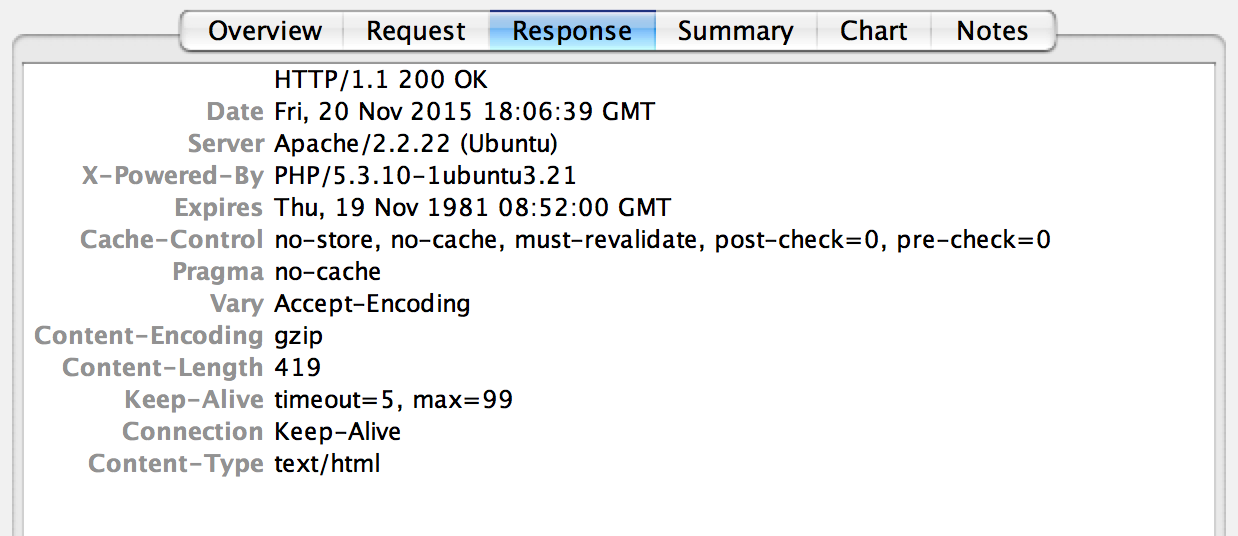
\includegraphics[scale=0.6]{figures/charles_results}
\end{figure}

\pagebreak

\pagebreak
\subsection{Test RIA cross domain policy (OTG-CONFIG-008)}\
\begin{tabular}{cR{12cm}}
	\textbf{Secode21} & Likelihood: 0\\& Impact: 0\\& Risk: 0
\end{tabular}

\begin{tabular}{ l|p{11cm}  }
	\hline
	\multicolumn{2}{c}{\textbf{Secode21}} \\
	\hline
	Observation   & There are no RIA applications on the system and therefore is no crossdomain.xml file provided. \\
	Discovery  & Using \textit{wget} we tried to find a \textit{crossdomain.xml} or \textit{clientaccesspolicy.xml} file and couldn't find it. \\
	Likelihood & N/A \\
	Implication    & N/A \\
	Recommendations & N/A \\
	Comparison & The same results applies for our web application. \\
	\hline
\end{tabular}
\\
\vspace{0.5cm}
\\
\begin{center}
	\begin{tabular}{ll}
		\rowcolor[HTML]{34CDF9}
		{\color[HTML]{ECF4FF} \textbf{Metric}}        & {\color[HTML]{ECF4FF} \textbf{Value}} \\
		\rowcolor[HTML]{BBDAFF}
		{\color[HTML]{333333} Access Vector}          & {\color[HTML]{333333} } N/A              \\
		\rowcolor[HTML]{ECF4FF}
		{\color[HTML]{333333} Attack Complexity}      & {\color[HTML]{333333} } N/A              \\
		\rowcolor[HTML]{BBDAFF}
		{\color[HTML]{333333} Privileges Required}    & {\color[HTML]{333333} } N/A              \\
		\rowcolor[HTML]{ECF4FF}
		{\color[HTML]{333333} User Interaction}       & {\color[HTML]{333333} } N/A              \\
		\rowcolor[HTML]{BBDAFF}
		{\color[HTML]{333333} Scope}                  & {\color[HTML]{333333} } N/A              \\
		\rowcolor[HTML]{ECF4FF}
		{\color[HTML]{333333} Confidentiality Impact} & {\color[HTML]{333333} } N/A              \\
		\rowcolor[HTML]{BBDAFF}
		{\color[HTML]{333333} Integrity Impact}       & {\color[HTML]{333333} } N/A              \\
		\rowcolor[HTML]{ECF4FF}
		{\color[HTML]{333333} Availability Impact}    & {\color[HTML]{333333} } N/A
	\end{tabular}
\end{center}
\pagebreak


\pagebreak
\section{Identity Management Testing}\
\subsection{Test Role Definitions (OTG-IDENT-001)}\
\begin{tabular}{cR{12cm}}
	\textbf{Secode21} & Likelihood: 10\\& Impact: 4\\& Risk: 4
\end{tabular}

\begin{tabular}{ l|p{11cm}  }
	\hline
	\multicolumn{2}{c}{\textbf{Secode21}} \\
	\hline
	Observation   & We found out that there exist two different roles in the system. There is the role of a normal customer and the role of an employee. Employees have the additional functionality to view account and transaction details of all the customers. Transactions over 10000 euro and new user registrations can be accepted by the employee. \\
	Discovery  & No special tools except a browser were needed because all the roles and their available functions are described. \\
	Likelihood & It is very likely that people find this information. \\
	Implication    & There is no direct implication, but knowing the roles and their functionality helps with other attacks. \\
	Recommendations & Don't describe the roles on the web page. \\
	Comparison & Our web application provides the same roles, but the roles are not described on the web page. \\
	\hline
\end{tabular}
\\
\vspace{0.5cm}
\\
\begin{center}
	\begin{tabular}{ll}
		\rowcolor[HTML]{34CDF9}
		{\color[HTML]{ECF4FF} \textbf{Metric}}        & {\color[HTML]{ECF4FF} \textbf{Value}} \\
		\rowcolor[HTML]{BBDAFF}
		{\color[HTML]{333333} Access Vector}          & {\color[HTML]{333333} } N              \\
		\rowcolor[HTML]{ECF4FF}
		{\color[HTML]{333333} Attack Complexity}      & {\color[HTML]{333333} } L              \\
		\rowcolor[HTML]{BBDAFF}
		{\color[HTML]{333333} Privileges Required}    & {\color[HTML]{333333} } L              \\
		\rowcolor[HTML]{ECF4FF}
		{\color[HTML]{333333} User Interaction}       & {\color[HTML]{333333} } N              \\
		\rowcolor[HTML]{BBDAFF}
		{\color[HTML]{333333} Scope}                  & {\color[HTML]{333333} } U              \\
		\rowcolor[HTML]{ECF4FF}
		{\color[HTML]{333333} Confidentiality Impact} & {\color[HTML]{333333} } L              \\
		\rowcolor[HTML]{BBDAFF}
		{\color[HTML]{333333} Integrity Impact}       & {\color[HTML]{333333} } L              \\
		\rowcolor[HTML]{ECF4FF}
		{\color[HTML]{333333} Availability Impact}    & {\color[HTML]{333333} } N
	\end{tabular}
\end{center}
\pagebreak

\subsection{Test User Registration Process (OTG-IDENT-002)}\
\begin{tabular}{cR{12cm}}
	\textbf{Secode21} & Likelihood: 5\\& Impact: 5\\& Risk: 5
\end{tabular}

\begin{tabular}{ l|p{11cm}  }
	\hline
	\multicolumn{2}{c}{\textbf{Secode21}} \\
	\hline
	Observation   & Any person can register themself as an user and this registration than gets validated by an employee. One person can register multiple times and with different roles. There is no proof of the identity of a user possible. The identification requirements include the name, surname, phone number, email address and username, but only two of these can be verified. \\
	Discovery  & No special tools are needed to get this information. A browser and multiple registration tests provided the necessary results. \\
	Likelihood & It is quite likely that this information can be retrieved by any user with minimal experience. \\
	Implication    & User could try to register multiple times and with wrong information to get access to user accounts with more permissions or to create multiple bank accounts. \\
	Recommendations & The information passed in the registration form should be validated, especially the email address and phone number can be verified very easily. The name can be validated by hand if a customer would go to the bank and the employee would than accept his registration. \\
	Comparison & Our web application doesn't require a phone number for the registration an the role of the user can be selected in the registration form. It doesn't make our application less secure, because the registration has still to be accepted by an employee. \\
	\hline
\end{tabular}
\\
\vspace{0.5cm}
\\
\begin{center}
	\begin{tabular}{ll}
		\rowcolor[HTML]{34CDF9}
		{\color[HTML]{ECF4FF} \textbf{Metric}}        & {\color[HTML]{ECF4FF} \textbf{Value}} \\
		\rowcolor[HTML]{BBDAFF}
		{\color[HTML]{333333} Access Vector}          & {\color[HTML]{333333} } N              \\
		\rowcolor[HTML]{ECF4FF}
		{\color[HTML]{333333} Attack Complexity}      & {\color[HTML]{333333} } L              \\
		\rowcolor[HTML]{BBDAFF}
		{\color[HTML]{333333} Privileges Required}    & {\color[HTML]{333333} } N              \\
		\rowcolor[HTML]{ECF4FF}
		{\color[HTML]{333333} User Interaction}       & {\color[HTML]{333333} } N              \\
		\rowcolor[HTML]{BBDAFF}
		{\color[HTML]{333333} Scope}                  & {\color[HTML]{333333} } U              \\
		\rowcolor[HTML]{ECF4FF}
		{\color[HTML]{333333} Confidentiality Impact} & {\color[HTML]{333333} } N              \\
		\rowcolor[HTML]{BBDAFF}
		{\color[HTML]{333333} Integrity Impact}       & {\color[HTML]{333333} } N              \\
		\rowcolor[HTML]{ECF4FF}
		{\color[HTML]{333333} Availability Impact}    & {\color[HTML]{333333} } N
	\end{tabular}
\end{center}
\pagebreak

\subsection{Test Account Provisioning Process (OTG-IDENT-003)}\
\begin{tabular}{cR{12cm}}
	\textbf{Secode21} & Likelihood: N/A\\& Impact: N/A\\& Risk: N/A
\end{tabular}

\begin{tabular}{ l|p{11cm}  }
	\hline
	\multicolumn{2}{c}{\textbf{Secode21}} \\
	\hline
	Observation   & Our observation showed us that employees can accept customer registrations and can make customer accounts to employee accounts. \\
	Discovery  & All the observations were made with the \textit{Chrome} web browser. \\
	Implication    & If an employee account gets hacked you can make even other accounts to employees and accept new registrations. \\
	Recommendations & N/A \\
	Comparison & In our web application the employee doesn't make customer accounts to employee accounts but rather accepts special employee registrations. It makes no difference in the security. \\
	\hline
\end{tabular}
\\
\vspace{0.5cm}
\\
\begin{center}
	\begin{tabular}{ll}
		\rowcolor[HTML]{34CDF9}
		{\color[HTML]{ECF4FF} \textbf{Metric}}        & {\color[HTML]{ECF4FF} \textbf{Value}} \\
		\rowcolor[HTML]{BBDAFF}
		{\color[HTML]{333333} Access Vector}          & {\color[HTML]{333333} } N              \\
		\rowcolor[HTML]{ECF4FF}
		{\color[HTML]{333333} Attack Complexity}      & {\color[HTML]{333333} } N/A              \\
		\rowcolor[HTML]{BBDAFF}
		{\color[HTML]{333333} Privileges Required}    & {\color[HTML]{333333} } N/A              \\
		\rowcolor[HTML]{ECF4FF}
		{\color[HTML]{333333} User Interaction}       & {\color[HTML]{333333} } N/A              \\
		\rowcolor[HTML]{BBDAFF}
		{\color[HTML]{333333} Scope}                  & {\color[HTML]{333333} } N/A              \\
		\rowcolor[HTML]{ECF4FF}
		{\color[HTML]{333333} Confidentiality Impact} & {\color[HTML]{333333} } N/A              \\
		\rowcolor[HTML]{BBDAFF}
		{\color[HTML]{333333} Integrity Impact}       & {\color[HTML]{333333} } N/A              \\
		\rowcolor[HTML]{ECF4FF}
		{\color[HTML]{333333} Availability Impact}    & {\color[HTML]{333333} } N/A
	\end{tabular}
\end{center}
\pagebreak

\subsection{Testing for Account Enumeration and Guessable User Account (OTG-IDENT-004)}\
\begin{tabular}{cR{12cm}}
	\textbf{Secode21} & Likelihood: 0\\& Impact: 0\\& Risk: 0
\end{tabular}

\begin{tabular}{ l|p{11cm}  }
	\hline
	\multicolumn{2}{c}{\textbf{Secode21}} \\
	\hline
	Observation   & We found out that the web application makes no difference between existing usernames and non existing usernames when trying to login with wrong credentials. The same html response and the same response headers are provided by the system. \\
	Discovery  & We used the \textit{Charles Web Proxy} to analyze the web application responses. \\
	Implication    & N/A \\
	Recommendations & N/A \\
	Comparison & Our web application makes no difference between login tries with existing usernames and non existing ones. Both web applications aren't vulnerable here. \\
	\hline
\end{tabular}
\\
\vspace{0.5cm}
\\
\begin{center}
	\begin{tabular}{ll}
		\rowcolor[HTML]{34CDF9}
		{\color[HTML]{ECF4FF} \textbf{Metric}}        & {\color[HTML]{ECF4FF} \textbf{Value}} \\
		\rowcolor[HTML]{BBDAFF}
		{\color[HTML]{333333} Access Vector}          & {\color[HTML]{333333} } N/A              \\
		\rowcolor[HTML]{ECF4FF}
		{\color[HTML]{333333} Attack Complexity}      & {\color[HTML]{333333} } N/A              \\
		\rowcolor[HTML]{BBDAFF}
		{\color[HTML]{333333} Privileges Required}    & {\color[HTML]{333333} } N/A              \\
		\rowcolor[HTML]{ECF4FF}
		{\color[HTML]{333333} User Interaction}       & {\color[HTML]{333333} } N/A              \\
		\rowcolor[HTML]{BBDAFF}
		{\color[HTML]{333333} Scope}                  & {\color[HTML]{333333} } N/A              \\
		\rowcolor[HTML]{ECF4FF}
		{\color[HTML]{333333} Confidentiality Impact} & {\color[HTML]{333333} } N/A              \\
		\rowcolor[HTML]{BBDAFF}
		{\color[HTML]{333333} Integrity Impact}       & {\color[HTML]{333333} } N/A              \\
		\rowcolor[HTML]{ECF4FF}
		{\color[HTML]{333333} Availability Impact}    & {\color[HTML]{333333} } N/A
	\end{tabular}
\end{center}
\pagebreak

\subsection{Testing for Weak or unenforced username policy (OTG-IDENT-005)}\
\begin{tabular}{cR{12cm}}
	\textbf{Secode21} & Likelihood: 0\\& Impact: 0\\& Risk: 0
\end{tabular}

\begin{tabular}{ l|p{11cm}  }
	\hline
	\multicolumn{2}{c}{\textbf{Secode21}} \\
	\hline
	Observation   & The usernames are not auto-generated and therefore there is no special structure in the usernames. \\
	Discovery  & No tool is used here. The username field in the registration form gives us all the information we need. \\
	Implication    & N/A \\
	Recommendations & N/A \\
	Comparison & The same applies for our web application. \\
	\hline
\end{tabular}
\\
\vspace{0.5cm}
\\
\begin{center}
	\begin{tabular}{ll}
		\rowcolor[HTML]{34CDF9}
		{\color[HTML]{ECF4FF} \textbf{Metric}}        & {\color[HTML]{ECF4FF} \textbf{Value}} \\
		\rowcolor[HTML]{BBDAFF}
		{\color[HTML]{333333} Access Vector}          & {\color[HTML]{333333} } N/A              \\
		\rowcolor[HTML]{ECF4FF}
		{\color[HTML]{333333} Attack Complexity}      & {\color[HTML]{333333} } N/A              \\
		\rowcolor[HTML]{BBDAFF}
		{\color[HTML]{333333} Privileges Required}    & {\color[HTML]{333333} } N/A              \\
		\rowcolor[HTML]{ECF4FF}
		{\color[HTML]{333333} User Interaction}       & {\color[HTML]{333333} } N/A              \\
		\rowcolor[HTML]{BBDAFF}
		{\color[HTML]{333333} Scope}                  & {\color[HTML]{333333} } N/A              \\
		\rowcolor[HTML]{ECF4FF}
		{\color[HTML]{333333} Confidentiality Impact} & {\color[HTML]{333333} } N/A              \\
		\rowcolor[HTML]{BBDAFF}
		{\color[HTML]{333333} Integrity Impact}       & {\color[HTML]{333333} } N/A              \\
		\rowcolor[HTML]{ECF4FF}
		{\color[HTML]{333333} Availability Impact}    & {\color[HTML]{333333} } N/A
	\end{tabular}
\end{center}
\pagebreak

\section{Authentication Testing}\
\subsection{Testing for Credentials Transported over an Encrypted Channel(OTG-AUTHN-001)}\

\begin{tabular}{cR{12cm}}
	\textbf{Secode21} & Likelihood: 8\\& Impact: 8\\& Risk: 8
\end{tabular}

\begin{tabular}{ l|p{11cm}  }
	\hline
	\multicolumn{2}{c}{\textbf{Secode21}} \\
	\hline
	Observation   & This ensures that our credentials are sent using an encrypted channel
	and that the credentials are not readable by a malicious user using a sniffer. The credetials are sent
	unencrypted over HTTP to the server and everyone in the network can read them.\\
	Discovery  &  We used \textit{Zed Attack Proxy (ZED)} in order to capture packet headers
	and to inspect them.  We saw that the request addressed to the web application is  using the HTTP protocol
	and that the credentials were simple POST parameters\\
	Likelihood & Everyone in the adjacent network or who can read the packages could also get the credentials \\
	Implication    & Authentication as user\\
	Recommendations & Use https to encrypt this information \\
	Comparison & The same applies for our web application.\\
	\hline
\end{tabular}
\\
\vspace{0.5cm}
\\
\begin{center}
	\begin{tabular}{ll}
		\rowcolor[HTML]{34CDF9}
		{\color[HTML]{ECF4FF} \textbf{Metric}}        & {\color[HTML]{ECF4FF} \textbf{Value}} \\
		\rowcolor[HTML]{BBDAFF}
		{\color[HTML]{333333} Access Vector}          & {\color[HTML]{333333} } A              \\
		\rowcolor[HTML]{ECF4FF}
		{\color[HTML]{333333} Attack Complexity}      & {\color[HTML]{333333} } L              \\
		\rowcolor[HTML]{BBDAFF}
		{\color[HTML]{333333} Privileges Required}    & {\color[HTML]{333333} } N              \\
		\rowcolor[HTML]{ECF4FF}
		{\color[HTML]{333333} User Interaction}       & {\color[HTML]{333333} } R              \\
		\rowcolor[HTML]{BBDAFF}
		{\color[HTML]{333333} Scope}                  & {\color[HTML]{333333} } U              \\
		\rowcolor[HTML]{ECF4FF}
		{\color[HTML]{333333} Confidentiality Impact} & {\color[HTML]{333333} } L              \\
		\rowcolor[HTML]{BBDAFF}
		{\color[HTML]{333333} Integrity Impact}       & {\color[HTML]{333333} } L              \\
		\rowcolor[HTML]{ECF4FF}
		{\color[HTML]{333333} Availability Impact}    & {\color[HTML]{333333} } N
	\end{tabular}
\end{center}

\pagebreak
\subsection{Testing for default credentials(OTG-AUTHN-002)}\
\begin{tabular}{cR{12cm}}
	\textbf{Secode21} & Likelihood: 10\\& Impact: 4\\& Risk: 6
\end{tabular}

\begin{tabular}{ l|p{11cm}  }
	\hline
	\multicolumn{2}{c}{\textbf{Secode21}} \\
	\hline
	Observation   & We found out that there exists the default credentials \textit{admin:admin} \\
	Discovery  & We were already given these credentials and additionally we tested the webapp with
	w3af where this credentials were discovered.\\
	Likelihood & It is very likely that people find this information. \\
	Implication    & The attacker gain employee access in the web application. \\
	Recommendations & Use other credentials for testing, or delete the default ones after you launch the application. \\
	Comparison & Our web application has a different combination of \textit{user:password}.\\
	\hline
\end{tabular}
\\
\vspace{0.5cm}
\\
\begin{center}
	\begin{tabular}{ll}
		\rowcolor[HTML]{34CDF9}
		{\color[HTML]{ECF4FF} \textbf{Metric}}        & {\color[HTML]{ECF4FF} \textbf{Value}} \\
		\rowcolor[HTML]{BBDAFF}
		{\color[HTML]{333333} Access Vector}          & {\color[HTML]{333333} } N              \\
		\rowcolor[HTML]{ECF4FF}
		{\color[HTML]{333333} Attack Complexity}      & {\color[HTML]{333333} } L              \\
		\rowcolor[HTML]{BBDAFF}
		{\color[HTML]{333333} Privileges Required}    & {\color[HTML]{333333} } N              \\
		\rowcolor[HTML]{ECF4FF}
		{\color[HTML]{333333} User Interaction}       & {\color[HTML]{333333} } N              \\
		\rowcolor[HTML]{BBDAFF}
		{\color[HTML]{333333} Scope}                  & {\color[HTML]{333333} } U              \\
		\rowcolor[HTML]{ECF4FF}
		{\color[HTML]{333333} Confidentiality Impact} & {\color[HTML]{333333} } L              \\
		\rowcolor[HTML]{BBDAFF}
		{\color[HTML]{333333} Integrity Impact}       & {\color[HTML]{333333} } L              \\
		\rowcolor[HTML]{ECF4FF}
		{\color[HTML]{333333} Availability Impact}    & {\color[HTML]{333333} } N
	\end{tabular}
\end{center}

\pagebreak
\subsection{Testing for bypassing authentication schema (OTG-AUTHN-004)}\

\begin{tabular}{cR{12cm}}
	\textbf{Secode21} & Likelihood: NA\\& Impact: NA\\& Risk: NA
\end{tabular}

\begin{tabular}{ l|p{11cm}  }
	\hline
	\multicolumn{2}{c}{\textbf{Secode21}} \\
	\hline
	Observation &  We did not find any possibility to bypass the authentication schema\\
	Discovery & NA\\
	Likelihood & NA\\
	Implication & NA\\
	Recommendations & NA\\
	Comparison & Neither we found a possibility in our web app \\
	\hline
\end{tabular}
\\
\vspace{0.5cm}
\\
\begin{center}
	\begin{tabular}{ll}
		\rowcolor[HTML]{34CDF9}
		{\color[HTML]{ECF4FF} \textbf{Metric}}        & {\color[HTML]{ECF4FF} \textbf{Value}} \\
		\rowcolor[HTML]{BBDAFF}
		{\color[HTML]{333333} Access Vector}          & {\color[HTML]{333333} } NA              \\
		\rowcolor[HTML]{ECF4FF}
		{\color[HTML]{333333} Attack Complexity}      & {\color[HTML]{333333} } NA              \\
		\rowcolor[HTML]{BBDAFF}
		{\color[HTML]{333333} Privileges Required}    & {\color[HTML]{333333} } NA              \\
		\rowcolor[HTML]{ECF4FF}
		{\color[HTML]{333333} User Interaction}       & {\color[HTML]{333333} } NA              \\
		\rowcolor[HTML]{BBDAFF}
		{\color[HTML]{333333} Scope}                  & {\color[HTML]{333333} } NA              \\
		\rowcolor[HTML]{ECF4FF}
		{\color[HTML]{333333} Confidentiality Impact} & {\color[HTML]{333333} } NA              \\
		\rowcolor[HTML]{BBDAFF}
		{\color[HTML]{333333} Integrity Impact}       & {\color[HTML]{333333} } NA              \\
		\rowcolor[HTML]{ECF4FF}
		{\color[HTML]{333333} Availability Impact}    & {\color[HTML]{333333} } NA
	\end{tabular}
\end{center}

\pagebreak
\subsection{Testing for Browser cache weakness (OTG-AUTHN-006)}\

\begin{tabular}{cR{12cm}}
	\textbf{Secode21} & Likelihood: 0\\& Impact: NA\\& Risk: NA
\end{tabular}

\begin{tabular}{ l|p{11cm}  }
	\hline
	\multicolumn{2}{c}{\textbf{Secode21}} \\
	\hline
	Observation & The web app set the cache-control to no-cache an no-store and Pragma to no-cache\\
	Discovery & By reviewing the response header with the chrome developer tools we could
	analyze the parameters\\
	Likelihood & For every registration process\\
	Implication & Brute Force is to easy for simple passwords\\
	Recommendations & Introduce password restrictions\\
	Comparison & The same problem we encountered in our webapp \\
	\hline
\end{tabular}
\\
\vspace{0.5cm}
\\
\begin{center}
	\begin{tabular}{ll}
		\rowcolor[HTML]{34CDF9}
		{\color[HTML]{ECF4FF} \textbf{Metric}}        & {\color[HTML]{ECF4FF} \textbf{Value}} \\
		\rowcolor[HTML]{BBDAFF}
		{\color[HTML]{333333} Access Vector}          & {\color[HTML]{333333} } NA              \\
		\rowcolor[HTML]{ECF4FF}
		{\color[HTML]{333333} Attack Complexity}      & {\color[HTML]{333333} } NA              \\
		\rowcolor[HTML]{BBDAFF}
		{\color[HTML]{333333} Privileges Required}    & {\color[HTML]{333333} } NA              \\
		\rowcolor[HTML]{ECF4FF}
		{\color[HTML]{333333} User Interaction}       & {\color[HTML]{333333} } NA              \\
		\rowcolor[HTML]{BBDAFF}
		{\color[HTML]{333333} Scope}                  & {\color[HTML]{333333} } NA              \\
		\rowcolor[HTML]{ECF4FF}
		{\color[HTML]{333333} Confidentiality Impact} & {\color[HTML]{333333} } NA              \\
		\rowcolor[HTML]{BBDAFF}
		{\color[HTML]{333333} Integrity Impact}       & {\color[HTML]{333333} } NA              \\
		\rowcolor[HTML]{ECF4FF}
		{\color[HTML]{333333} Availability Impact}    & {\color[HTML]{333333} } NA
	\end{tabular}
\end{center}

\pagebreak
\subsection{Testing for Weak password policy (OTG-AUTHN-007)}\

\begin{tabular}{cR{12cm}}
	\textbf{Secode21} & Likelihood: 6\\& Impact: 5\\& Risk: 5
\end{tabular}

\begin{tabular}{ l|p{11cm}  }
	\hline
	\multicolumn{2}{c}{\textbf{Secode21}} \\
	\hline
	Observation & The registration process does not have a restriction for weak passwords and the user can't
	change the password. Furthermore the password can contain the username\\
	Discovery & Tested manually the registration process with a one character password and the username as password\\
	Likelihood & For every registration process the user has the possibility to choose a weak password\\
	Implication & Brute Force is to easy for simple passwords\\
	Recommendations & Introduce password restrictions\\
	Comparison & The same problem we encountered in our webapp \\
	\hline
\end{tabular}
\\
\vspace{0.5cm}
\\
\begin{center}
	\begin{tabular}{ll}
		\rowcolor[HTML]{34CDF9}
		{\color[HTML]{ECF4FF} \textbf{Metric}}        & {\color[HTML]{ECF4FF} \textbf{Value}} \\
		\rowcolor[HTML]{BBDAFF}
		{\color[HTML]{333333} Access Vector}          & {\color[HTML]{333333} } N              \\
		\rowcolor[HTML]{ECF4FF}
		{\color[HTML]{333333} Attack Complexity}      & {\color[HTML]{333333} } L              \\
		\rowcolor[HTML]{BBDAFF}
		{\color[HTML]{333333} Privileges Required}    & {\color[HTML]{333333} } N              \\
		\rowcolor[HTML]{ECF4FF}
		{\color[HTML]{333333} User Interaction}       & {\color[HTML]{333333} } N              \\
		\rowcolor[HTML]{BBDAFF}
		{\color[HTML]{333333} Scope}                  & {\color[HTML]{333333} } U              \\
		\rowcolor[HTML]{ECF4FF}
		{\color[HTML]{333333} Confidentiality Impact} & {\color[HTML]{333333} } L              \\
		\rowcolor[HTML]{BBDAFF}
		{\color[HTML]{333333} Integrity Impact}       & {\color[HTML]{333333} } L              \\
		\rowcolor[HTML]{ECF4FF}
		{\color[HTML]{333333} Availability Impact}    & {\color[HTML]{333333} } N
	\end{tabular}
\end{center}

\pagebreak
\section{Authorization Testing}\
\subsection{Testing Directory traversal/file include (OTG-AUTHZ-001)}\

\begin{tabular}{cR{12cm}}
	\textbf{Secode21} & Likelihood: 4\\& Impact: 5\\& Risk: 5
\end{tabular}

\begin{tabular}{ l|p{11cm}  }
	\hline
	\multicolumn{2}{c}{\textbf{Secode21}} \\
	\hline
	Observation   & We could not find any path traversals with dotdotpwn but w3af found some.
	The phpinfo.php can be accessed and it contains the paths for several config files. So
	an attacker directly knows where to search for this files. Also since the attacker can see
	the phpinfo.php and see the installed software and its versions he can easily search for vulnerabilities for that version \\
	Discovery  & We used the dotdotpwn tool to find such traversals with the following command:
	\begin{lstlisting}
		sudo ./dotdotpwn.pl -O -m http -h 192.168.21.39
		-f /etc/hosts -k "localhost" -d 10 -s -E
	\end{lstlisting}
	-O is to get the operating system; -d 10 dotdotpwn will search until a deepness of 10;
	-m is to indicate that the protocol is http and -h for the server ip; -f /etc/hosts searches
	after the hosts file; -k defines that a file without ``localhost'' in it is a false positive.
	Afterwards we tried w3af and it found the phpinfo.php file\\
	Likelihood & This is more an additional information for other attacks but it is a
	good help for attackers to find vulnerabilities faster \\
	Implication    & The attacker knows the position of the config files, how php is
	configured and what version are used \\
	Recommendations & make the phpinfo page not accessible or delete it \\
	Comparison & Our webapp does not have a phpinfo page.\\
	\hline
\end{tabular}
\\
\vspace{0.5cm}
\\
\begin{center}
	\begin{tabular}{ll}
		\rowcolor[HTML]{34CDF9}
		{\color[HTML]{ECF4FF} \textbf{Metric}}        & {\color[HTML]{ECF4FF} \textbf{Value}} \\
		\rowcolor[HTML]{BBDAFF}
		{\color[HTML]{333333} Access Vector}          & {\color[HTML]{333333} } N              \\
		\rowcolor[HTML]{ECF4FF}
		{\color[HTML]{333333} Attack Complexity}      & {\color[HTML]{333333} } L              \\
		\rowcolor[HTML]{BBDAFF}
		{\color[HTML]{333333} Privileges Required}    & {\color[HTML]{333333} } N              \\
		\rowcolor[HTML]{ECF4FF}
		{\color[HTML]{333333} User Interaction}       & {\color[HTML]{333333} } N              \\
		\rowcolor[HTML]{BBDAFF}
		{\color[HTML]{333333} Scope}                  & {\color[HTML]{333333} } U              \\
		\rowcolor[HTML]{ECF4FF}
		{\color[HTML]{333333} Confidentiality Impact} & {\color[HTML]{333333} } L              \\
		\rowcolor[HTML]{BBDAFF}
		{\color[HTML]{333333} Integrity Impact}       & {\color[HTML]{333333} } N              \\
		\rowcolor[HTML]{ECF4FF}
		{\color[HTML]{333333} Availability Impact}    & {\color[HTML]{333333} } N
	\end{tabular}
\end{center}

\begin{figure}
	\centering
	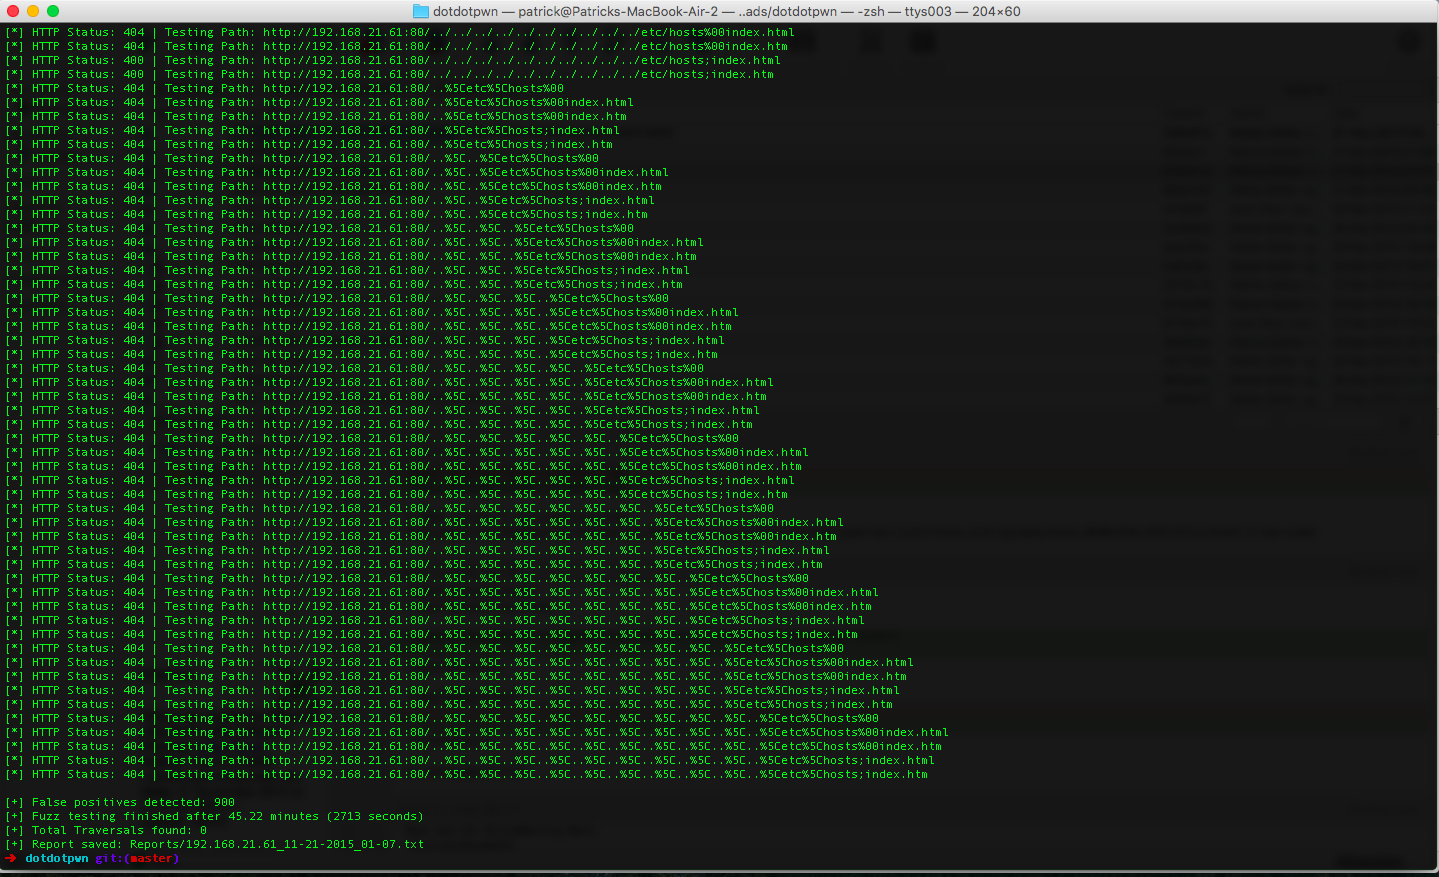
\includegraphics[width=\textwidth]{data/dotdotpwn.png}
	\caption{dotdotpwn screenshot}
	\label{fig:dotdotpwn}
\end{figure}

\pagebreak

\subsection{Testing for Privilege Escalation (OTG-AUTHZ-003)}\

\begin{tabular}{cR{12cm}}
	\textbf{Secode21} & Likelihood: 0\\& Impact: 0\\& Risk: 0
\end{tabular}

\begin{tabular}{ l|p{11cm}  }
	\hline
	\multicolumn{2}{c}{\textbf{Secode21}} \\
	\hline
	Observation   & It is not possible to escalate privileges of the user.  \\
	Discovery  & We tried to change the user privilege by changing the user id after we saw that they are generated by incrementing from the first user ID, using \textit{Burp}.\\
	Likelihood & N/A \\
	Implication    & N/A \\
	Recommendations & N/A \\
	Comparison & The same results apply for our web application.\\
	\hline
\end{tabular}

\pagebreak
\subsection{Testing for Insecure Direct Object References (OTG-AUTHZ-004)}\

\pagebreak
\section{Session Management Testing}\
\subsection{Testing for Bypassing Session Management Schema(OTG-SESS-001)}\

\begin{tabular}{cR{12cm}}
	\textbf{Secode21} & Likelihood: 0\\& Impact: 0\\& Risk: 0
\end{tabular}

\begin{tabular}{ l|p{11cm}  }
	\hline
	\multicolumn{2}{c}{\textbf{Secode21}} \\
	\hline
	Observation   & PHP session ids are used and such session ids normally can't be bypassed that means calculated easily\\
	Discovery  & We used the Chrome extension ``Advanced Rest Client'' to analyze the Request and the Cookies\\
	Likelihood & NA\\
	Implication    & NA\\
	Recommendations& NA\\
	Comparison& Our web application also uses PHP session ids \\
	\hline
\end{tabular}
\\
\vspace{0.5cm}
\\
\begin{center}
	\begin{tabular}{ll}
		\rowcolor[HTML]{34CDF9}
		{\color[HTML]{ECF4FF} \textbf{Metric}}        & {\color[HTML]{ECF4FF} \textbf{Value}} \\
		\rowcolor[HTML]{BBDAFF}
		{\color[HTML]{333333} Access Vector}          & {\color[HTML]{333333} } NA              \\
		\rowcolor[HTML]{ECF4FF}
		{\color[HTML]{333333} Attack Complexity}      & {\color[HTML]{333333} } NA              \\
		\rowcolor[HTML]{BBDAFF}
		{\color[HTML]{333333} Privileges Required}    & {\color[HTML]{333333} } NA              \\
		\rowcolor[HTML]{ECF4FF}
		{\color[HTML]{333333} User Interaction}       & {\color[HTML]{333333} } NA              \\
		\rowcolor[HTML]{BBDAFF}
		{\color[HTML]{333333} Scope}                  & {\color[HTML]{333333} } NA              \\
		\rowcolor[HTML]{ECF4FF}
		{\color[HTML]{333333} Confidentiality Impact} & {\color[HTML]{333333} } NA              \\
		\rowcolor[HTML]{BBDAFF}
		{\color[HTML]{333333} Integrity Impact}       & {\color[HTML]{333333} } NA              \\
		\rowcolor[HTML]{ECF4FF}
		{\color[HTML]{333333} Availability Impact}    & {\color[HTML]{333333} } NA
	\end{tabular}
\end{center}

\pagebreak
\subsection{Testing for Cookies attributes(OTG-SESS-002)}\

\begin{tabular}{cR{12cm}}
	\textbf{Secode21} & Likelihood: 10\\& Impact: 3\\& Risk: 3
\end{tabular}


\begin{tabular}{ l|p{11cm}  }
	\hline
	\multicolumn{2}{c}{\textbf{Secode21}} \\
	\hline
	Observation &  The cookie for the PHP session id has a to general path (``//''). So
	the application is vulnerable to other web application on the same server. They will
	also get the cookie from the user. \\

	Discovery  & We used the Chrome developer tools to analyze the cookies\\
	Likelihood & N/A\\
	Implication    & The cookies can be read and used by other web applications that
	match the path value. \\
	Recommendations & Set the path as thight as possible. For Team21 for example ``//secode//'' \\
	Comparison& Our web application has exact the same vulnerability.\\
	\hline
\end{tabular}
\\
\vspace{0.5cm}
\\
\begin{center}
	\begin{tabular}{ll}
		\rowcolor[HTML]{34CDF9}
		{\color[HTML]{ECF4FF} \textbf{Metric}}        & {\color[HTML]{ECF4FF} \textbf{Value}} \\
		\rowcolor[HTML]{BBDAFF}
		{\color[HTML]{333333} Access Vector}          & {\color[HTML]{333333} } L             \\
		\rowcolor[HTML]{ECF4FF}
		{\color[HTML]{333333} Attack Complexity}      & {\color[HTML]{333333} } L              \\
		\rowcolor[HTML]{BBDAFF}
		{\color[HTML]{333333} Privileges Required}    & {\color[HTML]{333333} } N              \\
		\rowcolor[HTML]{ECF4FF}
		{\color[HTML]{333333} User Interaction}       & {\color[HTML]{333333} } R              \\
		\rowcolor[HTML]{BBDAFF}
		{\color[HTML]{333333} Scope}                  & {\color[HTML]{333333} } U              \\
		\rowcolor[HTML]{ECF4FF}
		{\color[HTML]{333333} Confidentiality Impact} & {\color[HTML]{333333} } H              \\
		\rowcolor[HTML]{BBDAFF}
		{\color[HTML]{333333} Integrity Impact}       & {\color[HTML]{333333} } L              \\
		\rowcolor[HTML]{ECF4FF}
		{\color[HTML]{333333} Availability Impact}    & {\color[HTML]{333333} } N
	\end{tabular}
\end{center}

\pagebreak
\subsection{Testing for Session Fixation(OTG-SESS-003)}\

\begin{tabular}{cR{12cm}}
	\textbf{Secode21} & Likelihood: 8\\& Impact: 5\\& Risk: 5
\end{tabular}

\begin{tabular}{ l|p{11cm}  }
	\hline
	\multicolumn{2}{c}{\textbf{Secode21}} \\
	\hline
	Observation   & The session id is not invalidated and therefore does not change after the user is authenticated. This means
	an attacker can force a known session id on a user. Once the user is authenticated the attacker can access also as authenticated
	user \\
	Discovery  & We used the Chrome extension ``Advanced Rest Client'' to analyze the Request and the Cookies\\
	Likelihood & This attack is pretty easy and can also be performed by low skilled people\\
	Implication    & The attacker can do everything the user can \\
	Recommendations& Change the session id after logging in \\
	Comparison& Our web application has exact the same vulnerability\\
	\hline
\end{tabular}
\\
\vspace{0.5cm}
\\
\begin{center}
	\begin{tabular}{ll}
		\rowcolor[HTML]{34CDF9}
		{\color[HTML]{ECF4FF} \textbf{Metric}}        & {\color[HTML]{ECF4FF} \textbf{Value}} \\
		\rowcolor[HTML]{BBDAFF}
		{\color[HTML]{333333} Access Vector}          & {\color[HTML]{333333} } N             \\
		\rowcolor[HTML]{ECF4FF}
		{\color[HTML]{333333} Attack Complexity}      & {\color[HTML]{333333} } L              \\
		\rowcolor[HTML]{BBDAFF}
		{\color[HTML]{333333} Privileges Required}    & {\color[HTML]{333333} } N              \\
		\rowcolor[HTML]{ECF4FF}
		{\color[HTML]{333333} User Interaction}       & {\color[HTML]{333333} } R              \\
		\rowcolor[HTML]{BBDAFF}
		{\color[HTML]{333333} Scope}                  & {\color[HTML]{333333} } U              \\
		\rowcolor[HTML]{ECF4FF}
		{\color[HTML]{333333} Confidentiality Impact} & {\color[HTML]{333333} } H              \\
		\rowcolor[HTML]{BBDAFF}
		{\color[HTML]{333333} Integrity Impact}       & {\color[HTML]{333333} } H              \\
		\rowcolor[HTML]{ECF4FF}
		{\color[HTML]{333333} Availability Impact}    & {\color[HTML]{333333} } N
	\end{tabular}
\end{center}
\pagebreak
\subsection{Testing for Exposed Session Variables (OTG-SESS-004)}\

\begin{tabular}{cR{12cm}}
	\textbf{Secode21} & Likelihood: 10\\& Impact: 7\\& Risk: 7
\end{tabular}

\begin{tabular}{ l|p{11cm}  }
	\hline
	\multicolumn{2}{c}{\textbf{Secode21}} \\
	\hline
	Observation & The application from Team 21 does not use HTTPS and therefore the session variables
	are accessible during transport. An attacker could hijack the session simply read the session id by eavesdropping
	and reusing it \\
	Discovery & We used the Chrome developer tools to analyze the requests \\
	Likelihood & This attack is pretty easy and can also be performed by low skilled people\\
	Implication & The attacker can read the session variables and depending on the information in them  \\
	Recommendations & Use HTTP with TLS encryption and avoid GET request including the session id\\
	Comparison & Our web application has exact the same vulnerability\\
	\hline
\end{tabular}
\\
\vspace{0.5cm}
\\
\begin{center}
	\begin{tabular}{ll}
		\rowcolor[HTML]{34CDF9}
		{\color[HTML]{ECF4FF} \textbf{Metric}}        & {\color[HTML]{ECF4FF} \textbf{Value}} \\
		\rowcolor[HTML]{BBDAFF}
		{\color[HTML]{333333} Access Vector}          & {\color[HTML]{333333} } A             \\
		\rowcolor[HTML]{ECF4FF}
		{\color[HTML]{333333} Attack Complexity}      & {\color[HTML]{333333} } L              \\
		\rowcolor[HTML]{BBDAFF}
		{\color[HTML]{333333} Privileges Required}    & {\color[HTML]{333333} } N              \\
		\rowcolor[HTML]{ECF4FF}
		{\color[HTML]{333333} User Interaction}       & {\color[HTML]{333333} } R              \\
		\rowcolor[HTML]{BBDAFF}
		{\color[HTML]{333333} Scope}                  & {\color[HTML]{333333} } U              \\
		\rowcolor[HTML]{ECF4FF}
		{\color[HTML]{333333} Confidentiality Impact} & {\color[HTML]{333333} } H              \\
		\rowcolor[HTML]{BBDAFF}
		{\color[HTML]{333333} Integrity Impact}       & {\color[HTML]{333333} } H              \\
		\rowcolor[HTML]{ECF4FF}
		{\color[HTML]{333333} Availability Impact}    & {\color[HTML]{333333} } N
	\end{tabular}
\end{center}

\pagebreak
\subsection{Testing for Cross Site Request Forgery (OTG-SESS-005)}\


\pagebreak
\subsection{Testing for logout functionality(OTG-SESS-006)}\

\begin{tabular}{cR{12cm}}
	\textbf{Secode21} & Likelihood: 5\\& Impact: 6\\& Risk: 5
\end{tabular}

\begin{tabular}{ l|p{11cm}  }
	\hline
	\multicolumn{2}{c}{\textbf{Secode21}} \\
	\hline
	Observation & The logout functionallity has been tested an works without any problems.
	The user gets correctly logged out and pages where authentication is needed can't be accessed afterwards.
	Also reusing the session id does not work. But the application seems to have no automatic
	logout after a certain amount of time.\\
	Discovery & We tested the functionallity manually and used the Chrome extension ``Advanced Rest Client''
	to reuse the session cookie \\
	Likelihood & The only problem is that user sometimes only close the browser tab and than the session continues to exist\\
	Implication & An attacker would be logged in if he can access afterwards the computer. Possible scenario Internet cafe
	or something similar\\
	Recommendations & implement an automatic server side logout\\
	Comparison & Our web application works also as expected but also does not have an automatic logout on the server side\\
	\hline
\end{tabular}
\\
\vspace{0.5cm}
\\
\begin{center}
	\begin{tabular}{ll}
		\rowcolor[HTML]{34CDF9}
		{\color[HTML]{ECF4FF} \textbf{Metric}}        & {\color[HTML]{ECF4FF} \textbf{Value}} \\
		\rowcolor[HTML]{BBDAFF}
		{\color[HTML]{333333} Access Vector}          & {\color[HTML]{333333} } P             \\
		\rowcolor[HTML]{ECF4FF}
		{\color[HTML]{333333} Attack Complexity}      & {\color[HTML]{333333} } L              \\
		\rowcolor[HTML]{BBDAFF}
		{\color[HTML]{333333} Privileges Required}    & {\color[HTML]{333333} } N              \\
		\rowcolor[HTML]{ECF4FF}
		{\color[HTML]{333333} User Interaction}       & {\color[HTML]{333333} } N              \\
		\rowcolor[HTML]{BBDAFF}
		{\color[HTML]{333333} Scope}                  & {\color[HTML]{333333} } U              \\
		\rowcolor[HTML]{ECF4FF}
		{\color[HTML]{333333} Confidentiality Impact} & {\color[HTML]{333333} } N              \\
		\rowcolor[HTML]{BBDAFF}
		{\color[HTML]{333333} Integrity Impact}       & {\color[HTML]{333333} } H              \\
		\rowcolor[HTML]{ECF4FF}
		{\color[HTML]{333333} Availability Impact}    & {\color[HTML]{333333} } N
	\end{tabular}
\end{center}

\pagebreak
\subsection{Test Session Timeout(OTG-SESS-007)}\

\begin{tabular}{cR{12cm}}
	\textbf{Secode21} & Likelihood: 4\\& Impact: 6\\& Risk: 7
\end{tabular}

\begin{tabular}{ l|p{11cm}  }
	\hline
	\multicolumn{2}{c}{\textbf{Secode21}} \\
	\hline
	Observation & The application has the timeout of the session set to the browsers
	session lifetime.\\
	Discovery & We tested the functionallity manually and used the Chrome developertools to check the cookies\\
	Likelihood & same as for OTG-SESS-006. Public computers are here the biggest problem\\
	Implication & An attacker is directly authenticated if the session is not ended\\
	Recommendations & Implement a server side session invalidation and delete the stored data on the client\\
	Comparison & Also our webapp has this vulnerability\\
	\hline
\end{tabular}
\\
\vspace{0.5cm}
\\
\begin{center}
	\begin{tabular}{ll}
		\rowcolor[HTML]{34CDF9}
		{\color[HTML]{ECF4FF} \textbf{Metric}}        & {\color[HTML]{ECF4FF} \textbf{Value}} \\
		\rowcolor[HTML]{BBDAFF}
		{\color[HTML]{333333} Access Vector}          & {\color[HTML]{333333} } P             \\
		\rowcolor[HTML]{ECF4FF}
		{\color[HTML]{333333} Attack Complexity}      & {\color[HTML]{333333} } L              \\
		\rowcolor[HTML]{BBDAFF}
		{\color[HTML]{333333} Privileges Required}    & {\color[HTML]{333333} } N              \\
		\rowcolor[HTML]{ECF4FF}
		{\color[HTML]{333333} User Interaction}       & {\color[HTML]{333333} } N              \\
		\rowcolor[HTML]{BBDAFF}
		{\color[HTML]{333333} Scope}                  & {\color[HTML]{333333} } U              \\
		\rowcolor[HTML]{ECF4FF}
		{\color[HTML]{333333} Confidentiality Impact} & {\color[HTML]{333333} } N              \\
		\rowcolor[HTML]{BBDAFF}
		{\color[HTML]{333333} Integrity Impact}       & {\color[HTML]{333333} } H              \\
		\rowcolor[HTML]{ECF4FF}
		{\color[HTML]{333333} Availability Impact}    & {\color[HTML]{333333} } N
	\end{tabular}
\end{center}

\pagebreak
\subsection{Testing for Session puzzling(OTG-SESS-008)}\

\begin{tabular}{cR{12cm}}
	\textbf{Secode21} & Likelihood: 0\\& Impact: 0\\& Risk: 0
\end{tabular}

\begin{tabular}{ l|p{11cm}  }
	\hline
	\multicolumn{2}{c}{\textbf{Secode21}} \\
	\hline
	Observation & The application has only one authorization method so a session puzzling
	is not applicable.\\
	Discovery & Manually searched\\
	Likelihood & NA\\
	Implication & NA\\
	Recommendations & NA\\
	Comparison & We provide also only one possibility to login so session puzzling is not possible\\
	\hline
\end{tabular}

\pagebreak
\section{Data Validation Testing}\
\subsection{Testing for Reflected Cross Site Scripting(OTG-INPVAL-001)}\

\begin{tabular}{cc}
	\textbf{Secode21} \hspace{9cm} & \begin{tabular}{@{}c@{}c@{}}Likelihood: 8\\ Impact: 5\\ Risk:5 \end{tabular}
\end{tabular}\

\begin{tabular}{ l|p{11cm}  }
	\hline
	\multicolumn{2}{c}{\textbf{Secode21}} \\
	\hline
	Observation   & We observed no reflected cross site scripting vulnerability. \\
	Discovery  & It seems that all parameters are stored in the database before inserting the values in the HTML. \\
	Likelihood & N/A \\
	Implication    & N/A \\
	Recommendations &  N/A \\
	Comparison& The same results apply for our web application. \\
	\hline
\end{tabular}

\pagebreak
\subsection{Testing for Stored Cross Site Scripting(OTG-INPVAL-002)}\

\begin{tabular}{cc}
	\textbf{Secode21} \hspace{9cm} & \begin{tabular}{@{}c@{}c@{}}Likelihood: 8\\ Impact: 5\\ Risk:5 \end{tabular}
\end{tabular}\

\begin{tabular}{ l|p{11cm}  }
	\hline
	\multicolumn{2}{c}{\textbf{Secode21}} \\
	\hline
	Observation   &  We observed several possibilities to execute a stored XSS attack. But not all of
	them could be exploited as the length of the corresponding database fields was
	often very restricted.
	We manually tried to inject JavaScript code in every input field. Therefore we
	used the following code, which just alerts a message.
	\begin{lstlisting}
		<script type="javascript">alert("XSS");</script>
	\end{lstlisting} \\
	Discovery  & We inserted Javascript code in the name field on the register page.
	When we logged in as an employee the script was executed.  There were cases when the script caused for new registered users after the script was entered to not appear. \\
	Likelihood & This vulnerability can be easily detected, but require some JavaScript knowledge to exploit it. Therefore we estimated the likelihood to be medium. \\
	Implication    & The implications are severe as we proofed that it is possible to steal the session. As we injected the code on the admin landingpage, which implies that we were able to act as an admin and register an abitrary account. \\
	Recommendations & Implement a input sanitation on all input fields on the backend side!  Try to use whitelisting for the different datatypes and do not rely on the frontend input
	validation. \\
	Comparison& \\
	\hline
\end{tabular}

\vspace{0.5cm}
\begin{center}
	% Please add the following required packages to your document preamble:
	% \usepackage[table,xcdraw]{xcolor}
	% If you use beamer only pass "xcolor=table" option, i.e. \documentclass[xcolor=table]{beamer}
	%\begin{table}[]
	%\centering
	%	\caption{My caption}
	%\label{my-label}
	\begin{tabular}{ll}
		\rowcolor[HTML]{34CDF9}
		{\color[HTML]{ECF4FF} \textbf{Metric}}        & {\color[HTML]{ECF4FF} \textbf{Value}} \\
		\rowcolor[HTML]{BBDAFF}
		{\color[HTML]{333333} Access Vector}          & {\color[HTML]{333333} N}               \\
		\rowcolor[HTML]{ECF4FF}
		{\color[HTML]{333333} Attack Complexity}      & {\color[HTML]{333333} M}               \\
		\rowcolor[HTML]{BBDAFF}
		{\color[HTML]{333333} Privileges Required}    & {\color[HTML]{333333} N}               \\
		\rowcolor[HTML]{ECF4FF}
		{\color[HTML]{333333} User Interaction}       & {\color[HTML]{333333} Y}               \\
		\rowcolor[HTML]{BBDAFF}
		{\color[HTML]{333333} Scope}                  & {\color[HTML]{333333} U}               \\
		\rowcolor[HTML]{ECF4FF}
		{\color[HTML]{333333} Confidentiality Impact} & {\color[HTML]{333333} M}               \\
		\rowcolor[HTML]{BBDAFF}
		{\color[HTML]{333333} Integrity Impact}       & {\color[HTML]{333333} M}               \\
		\rowcolor[HTML]{ECF4FF}
		{\color[HTML]{333333} Availability Impact}    & {\color[HTML]{333333} L}
	\end{tabular}
	%\end{table}
\end{center}
\pagebreak
\subsection{Testing for HTTP Verb Tampering(OTG-INPVAL-003)}\


\begin{tabular}{cR{12cm}}
	\textbf{Secode21} & Likelihood: 0\\& Impact: 0\\& Risk: 0
\end{tabular}

\begin{tabular}{ l|p{11cm}  }
	\hline
	\multicolumn{2}{c}{\textbf{Secode21}} \\
	\hline
	Observation   &  We did not observe any notable behavior.  \\
	Discovery  &  We used the Zed  Attack  Proxy  (ZAP)	to change the HTTP requests method to the ones listed below. The requests that were allowed responded
	with the index page or an empty body. The rejected requests responded with an
	error message in the body.\

	Methods that were allowed\

	\begin{itemize}
		\item HEAD
		\item OPTIONS
		\item GET
		\item POST

	\end{itemize}

	Methods that were rejected\

	\begin{itemize}
		\item TRACE
		\item PUT
		\item PROPFIND
	\end{itemize} \\

	Likelihood & N/A \\
	Implication    & N/A \\
	Recommendations & N/A \\
	Comparison &  Both webapps have the same allowed methods.\\
	\hline
\end{tabular}

\begin{figure}
	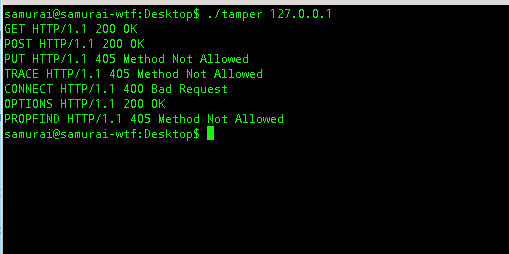
\includegraphics[width=\linewidth]{tampering.png}
	\caption{Results}
	\label{fig:test}
\end{figure}

\begin{figure}
	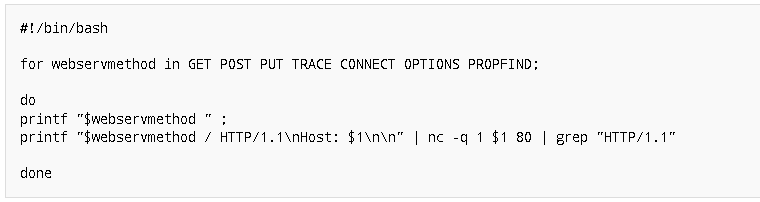
\includegraphics[width=\linewidth]{script.png}
	\caption{Script used for testing}
	\label{fig:script}
\end{figure}

\pagebreak
\subsection{Testing for SQL Injection (OTG-INPVAL-005) and Mysql testing (OTG-INPVAL-005)}\

\begin{tabular}{cR{12cm}}
	\textbf{Secode21} & Likelihood: 0\\& Impact: 0\\& Risk: 0
\end{tabular}

\begin{tabular}{ l|p{11cm}  }
	\hline
	\multicolumn{2}{c}{\textbf{Secode21}} \\
	\hline
	Observation   & We observed that no SQL Injection was possible. Since we knew that the other team had
	to use Mysql we tested also specifically for Mysql \\
	Discovery  & We tried inserting various SQL statements in the fields of using \textit{SQL Inject Me} tool and failed.
	Also w3af was used and it could not find any vulnerabilities \\
	Likelihood & N/A \\
	Implication    & N/A \\
	Recommendations & N/A \\
	Comparison& Our web application is also immune to SQL Injections \\
	\hline
\end{tabular}

\pagebreak
\subsection{Testing for XML Injection(OTG-INPVAL-008)}\

\begin{tabular}{cR{12cm}}
	\textbf{Secode21} & Likelihood: 0\\& Impact: 0\\& Risk: 0
\end{tabular}

\begin{tabular}{ l|p{11cm}  }
	\hline
	\multicolumn{2}{c}{\textbf{Secode21}} \\
	\hline
	Observation   & We did not find any vulnerability regarding XML Injection\\
	Discovery  & We used w3af to find XML injection vulerabilities and it could not find any. \\
	Likelihood & N/A \\
	Implication    & N/A \\
	Recommendations & N/A \\
	Comparison& Our web application is also immune to XML Injections \\
	\hline
\end{tabular}

\pagebreak
\subsection{Testing for SSI Injection(OTG-INPVAL-009)}\

\begin{tabular}{cR{12cm}}
	\textbf{Secode21} & Likelihood: 0\\& Impact: 0\\& Risk: 0
\end{tabular}

\begin{tabular}{ l|p{11cm}  }
	\hline
	\multicolumn{2}{c}{\textbf{Secode21}} \\
	\hline
	Observation   & We did not find any vulnerability regarding SSI Injection\\
	Discovery  & We used w3af to find SSI injection possibilities and it could not find any vulnerabilities. \\
	Likelihood & N/A \\
	Implication    & N/A \\
	Recommendations & N/A \\
	Comparison& Our web application is also immune to XML Injections \\
	\hline
\end{tabular}

\pagebreak
\subsection{Testing for XPATH Injection(OTG-INPVAL-010)}\

\begin{tabular}{cR{12cm}}
	\textbf{Secode21} & Likelihood: 0\\& Impact: 0\\& Risk: 0
\end{tabular}

\begin{tabular}{ l|p{11cm}  }
	\hline
	\multicolumn{2}{c}{\textbf{Secode21}} \\
	\hline
	Observation   & We did not find any vulnerability regarding XPATH Injection\\
	Discovery  & We used w3af to find XPATH injections and it could not find any vulnerabilities \\
	Likelihood & N/A \\
	Implication    & N/A \\
	Recommendations & N/A \\
	Comparison& Our web application is also immune to XPATH Injections \\
	\hline
\end{tabular}

\pagebreak
\subsection{Testing for Code Injection, Testing for Local File Inclusion, Testing for Remote File Inclusion(OTG-INPVAL-012)}\

\begin{tabular}{cR{12cm}}
	\textbf{Secode21} & Likelihood: 0\\& Impact: 0\\& Risk: 0
\end{tabular}

\begin{tabular}{ l|p{11cm}  }
	\hline
	\multicolumn{2}{c}{\textbf{Secode21}} \\
	\hline
	Observation   & We did not find any vulnerability regarding code injection and local or remote file inclusion in our
	web app. Team 21 did not implemented that feature\\
	Discovery  & Tryed to perform a command execution via the backticks (`) and also the semicolon (;) in the filename but our
	webapp correctly handled the files without injections \\
	Likelihood & N/A \\
	Implication    & N/A \\
	Recommendations & N/A \\
	Comparison& NA \\
	\hline
\end{tabular}

\pagebreak
\subsection{Testing for Command Injection(OTG-INPVAL-013)}\

\begin{tabular}{cR{12cm}}
	\textbf{Secode21} & Likelihood: 0\\& Impact: 0\\& Risk: 0
\end{tabular}

\begin{tabular}{ l|p{11cm}  }
	\hline
	\multicolumn{2}{c}{\textbf{Secode21}} \\
	\hline
	Observation   & Could not find any possibilities too for such a injection\\
	Discovery  & Searched manually and used the OWASPTOP10 profile for w3af and did not found a possibility\\
	Likelihood & N/A \\
	Implication    & N/A \\
	Recommendations & N/A \\
	Comparison& Neither our app showed such a vulnerability\\
	\hline
\end{tabular}

\pagebreak
\subsection{Testing for Buffer overflow, Testing for Heap overflow, Testing for Stack overflow, Testing for Format string (OTG-INPVAL-014)}\

\begin{tabular}{cR{12cm}}
	\textbf{Secode21} & Likelihood: 0\\& Impact: 0\\& Risk: 0
\end{tabular}

\begin{tabular}{ l|p{11cm}  }
	\hline
	\multicolumn{2}{c}{\textbf{Secode21}} \\
	\hline
	Observation   & We did not find any vulnerability regarding buffer overflow,
	heap overflow, stack overflow or string formatting\\
	Discovery  & We used w3af to locate such vilnerabilities. \\
	Likelihood & N/A \\
	Implication    & N/A \\
	Recommendations & N/A \\
	Comparison& Our web application is also immune to buffer overflow,
	heap overflow, stack overflow and string formatting \\
	\hline
\end{tabular}

\pagebreak
\subsection{Testing for incubated vulnerabilities(OTG-INPVAL-015)}\

\begin{tabular}{cR{12cm}}
	\textbf{Secode21} & Likelihood: 7\\& Impact: 7\\& Risk: 5
\end{tabular}

\begin{tabular}{ l|p{11cm}  }
	\hline
	\multicolumn{2}{c}{\textbf{Secode21}} \\
	\hline
	Observation   & A part of the XSS injection counts also to this vulnerability thats possible on the web app of
	team 21. Code like the example on the owasp page for OTG-INPVAL-015 could exploit the web app\\
	Discovery  & We knew that stored XSS is possible so also this attack works and someone could hijack an
	admins account simply by creating an user\\
	Likelihood & The attack is pretty easy and the employee only has to view the accounts
	page and if the attacker is a bit skilled the employee does not even discover that something was wrong \\
	Implication    & The attacker can hijack the session and do all the other things possible with XSS\\
	Recommendations & Validate and escape the user input \\
	Comparison& Our web application has the same vulnerability but there it is a lot more restricted.
	Only really short injection code can be used so the possibilities are limited. \\
	\hline
\end{tabular}

\section{Error Handling}\

\textbf{Team21}\\

Team21 does not provide a lot of error messages for incorrect inputs (e.g. incorrect TAN
length, wrong TAN, TAN used). \\
Based on the client side input validation, there are also no messages for manipulated input via proxy or by removing the validation patterns, which can lead to problems. Examples would be a malformated email which results in a not working account or a longer input then expected, which cuts off the end of the input. There are some cases when the page returns the path of the file where the error occurred.\\

\textbf{Team3}\\


\section{Cryptography}\

\pagebreak
\section{Business Logic Testing}\
\subsection{Test Business Logic Data Validation(OTG-BUSLOGIC-001)}\

\begin{tabular}{cc}
	\textbf{Secode21} \hspace{9cm} & \begin{tabular}{@{}c@{}c@{}}Likelihood: 0\\ Impact: 0\\ Risk:0 \end{tabular}
\end{tabular}\

\begin{tabular}{ l|p{11cm}  }
	\hline
	\multicolumn{2}{c}{\textbf{Secode21}} \\
	\hline
	Observation   & Tests show that data validation is both: client side and server side.\\
	Discovery  & We intercepted the input before it gets send to the server using \textit{Burp} and manipulated the data, and we received an error message. \\

	Likelihood & N/A \\
	Implication    & N/A \\
	Recommendations & N/A \\
	Comparison& We got the same result with our application. \\
	\hline
\end{tabular}

\pagebreak
\subsection{Test Ability to Forge Requests(OTG-BUSLOGIC-002)}\
\pagebreak
\subsection{Test Integrity Checks(OTG-BUSLOGIC-003)}\
\pagebreak
\subsection{Test for Process Timing(OTG-BUSLOGIC-004)}\
\pagebreak
\subsection{Test Number of Times a Function Can be Used Limits(OTG-BUSLOGIC-005)}\

\begin{tabular}{cc}
	\textbf{Secode21} \hspace{9cm} & \begin{tabular}{@{}c@{}c@{}}Likelihood: 0\\ Impact: 0\\ Risk:0 \end{tabular}
\end{tabular}\

\begin{tabular}{ l|p{11cm}  }
	\hline
	\multicolumn{2}{c}{\textbf{Secode21}} \\
	\hline
	Observation   & We tried inserting the same tan multiple times.\\
	Discovery  & The web application did not accept requests with a TAN that was already used. \\

	Likelihood & N/A \\
	Implication    & N/A \\
	Recommendations & N/A \\
	Comparison& We got the same result with our application. \\
	\hline
\end{tabular}

\pagebreak
\subsection{Testing for the Circumvention of Work Flows(OTG-BUSLOGIC-006)}\
\pagebreak
\subsection{Test Defenses Against Application Misuse(OTG-BUSLOGIC-007)}\
\pagebreak
\subsection{Test Upload of Unexpected File Types(OTG-BUSLOGIC-008)}\
\pagebreak
\subsection{Test Upload of Malicious Files(OTG-BUSLOGIC-009)}\
\pagebreak

\section{Client Side Testing}

\subsection{Testing for DOM based Cross Site Scripting (OTG-CLIENT-001)}\

\begin{tabular}{cR{12cm}}
	\textbf{Secode21} & Likelihood: 0\\& Impact: 0\\& Risk: 0
\end{tabular}

\begin{tabular}{ l|p{11cm}  }
	\hline
	\multicolumn{2}{c}{\textbf{Secode21}} \\
	\hline
	Observation   & Observing the HTML source code showed us that they don't use javascript and therefore there can't be any DOM XSS vulnerabilities. \\
	Discovery  & We used \textit{Chrome} and its developer tools to take a look at the HTML source code. \\
	Likelihood & N/A \\
	Implication    & N/A \\
	Comparison & Our web application uses javascript in many different cases, but we couldn't find any DOM XSS vulnerabilities. \\
	\hline
\end{tabular}
\\
\vspace{0.5cm}
\\
\begin{center}
	\begin{tabular}{ll}
		\rowcolor[HTML]{34CDF9}
		{\color[HTML]{ECF4FF} \textbf{Metric}}        & {\color[HTML]{ECF4FF} \textbf{Value}} \\
		\rowcolor[HTML]{BBDAFF}
		{\color[HTML]{333333} Access Vector}          & {\color[HTML]{333333} } N/A              \\
		\rowcolor[HTML]{ECF4FF}
		{\color[HTML]{333333} Attack Complexity}      & {\color[HTML]{333333} } N/A              \\
		\rowcolor[HTML]{BBDAFF}
		{\color[HTML]{333333} Privileges Required}    & {\color[HTML]{333333} } N/A              \\
		\rowcolor[HTML]{ECF4FF}
		{\color[HTML]{333333} User Interaction}       & {\color[HTML]{333333} } N/A              \\
		\rowcolor[HTML]{BBDAFF}
		{\color[HTML]{333333} Scope}                  & {\color[HTML]{333333} } N/A              \\
		\rowcolor[HTML]{ECF4FF}
		{\color[HTML]{333333} Confidentiality Impact} & {\color[HTML]{333333} } N/A              \\
		\rowcolor[HTML]{BBDAFF}
		{\color[HTML]{333333} Integrity Impact}       & {\color[HTML]{333333} } N/A              \\
		\rowcolor[HTML]{ECF4FF}
		{\color[HTML]{333333} Availability Impact}    & {\color[HTML]{333333} } N/A
	\end{tabular}
\end{center}

\pagebreak

\subsection{Testing for JavaScript Execution (OTG-CLIENT-002)}\
\begin{tabular}{cR{12cm}}
	\textbf{Secode21} & Likelihood: 9\\& Impact: 10\\& Risk: 9
\end{tabular}

\begin{tabular}{ l|p{11cm}  }
	\hline
	\multicolumn{2}{c}{\textbf{Secode21}} \\
	\hline
	Observation   & We found several XSS vulnerabilities allowing the execution of arbitrary javascript code in the clients browser. \\
	Discovery  & We used the tools \textit{w3af} and \textit{ZED Attack Proxy} to find some XSS vulnerabilities and found enough of them. \\
	Likelihood & It is very likely that these vulnerabilities are found and you don't need much experience to use them. \\
	Implication    & The vulnerabilities found can be used to hijack the session of an user, accept user registrations or even making user accounts to employee accounts. \\
	Comparison & Our app is also vulnerable against XSS attacks but the difficulty is higher as in their web application. More experienced people are necessary to exploit them. \\
	\hline
\end{tabular}
\\
\vspace{0.5cm}
\\
\begin{center}
	\begin{tabular}{ll}
		\rowcolor[HTML]{34CDF9}
		{\color[HTML]{ECF4FF} \textbf{Metric}}        & {\color[HTML]{ECF4FF} \textbf{Value}} \\
		\rowcolor[HTML]{BBDAFF}
		{\color[HTML]{333333} Access Vector}          & {\color[HTML]{333333} } N              \\
		\rowcolor[HTML]{ECF4FF}
		{\color[HTML]{333333} Attack Complexity}      & {\color[HTML]{333333} } L              \\
		\rowcolor[HTML]{BBDAFF}
		{\color[HTML]{333333} Privileges Required}    & {\color[HTML]{333333} } N              \\
		\rowcolor[HTML]{ECF4FF}
		{\color[HTML]{333333} User Interaction}       & {\color[HTML]{333333} } N              \\
		\rowcolor[HTML]{BBDAFF}
		{\color[HTML]{333333} Scope}                  & {\color[HTML]{333333} } U              \\
		\rowcolor[HTML]{ECF4FF}
		{\color[HTML]{333333} Confidentiality Impact} & {\color[HTML]{333333} } H              \\
		\rowcolor[HTML]{BBDAFF}
		{\color[HTML]{333333} Integrity Impact}       & {\color[HTML]{333333} } H              \\
		\rowcolor[HTML]{ECF4FF}
		{\color[HTML]{333333} Availability Impact}    & {\color[HTML]{333333} } L
	\end{tabular}
\end{center}
\pagebreak

\subsection{Testing for HTML Injection (OTG-CLIENT-003)}\
\begin{tabular}{cR{12cm}}
	\textbf{Secode21} & Likelihood: 8\\& Impact: 7\\& Risk: 7
\end{tabular}

\begin{tabular}{ l|p{11cm}  }
	\hline
	\multicolumn{2}{c}{\textbf{Secode21}} \\
	\hline
	Observation   & The HTML injection vulnerability exists  \\
	Discovery  & The vulnerability was found by the tools \textit{w3af} and \textit{ZED Attack Proxy}. \\
	Likelihood & It is quite likely that this vulnerability is found and can be used very easily. \\
	Implication    &  vulnerability can have many consequences, like disclosure of a user's session cookies that could be used to impersonate the victim, or, more generally, it can allow the attacker to modify the page content seen by the victims. \\
	Comparison & Our web application is vulnerable as well, but javascript validations and text length restrictions of the input fields make it more difficult to exploit these vulnerabilities. \\
	\hline
\end{tabular}
\\
\vspace{0.5cm}
\\
\begin{center}
	\begin{tabular}{ll}
		\rowcolor[HTML]{34CDF9}
		{\color[HTML]{ECF4FF} \textbf{Metric}}        & {\color[HTML]{ECF4FF} \textbf{Value}} \\
		\rowcolor[HTML]{BBDAFF}
		{\color[HTML]{333333} Access Vector}          & {\color[HTML]{333333} } N              \\
		\rowcolor[HTML]{ECF4FF}
		{\color[HTML]{333333} Attack Complexity}      & {\color[HTML]{333333} } L              \\
		\rowcolor[HTML]{BBDAFF}
		{\color[HTML]{333333} Privileges Required}    & {\color[HTML]{333333} } N              \\
		\rowcolor[HTML]{ECF4FF}
		{\color[HTML]{333333} User Interaction}       & {\color[HTML]{333333} } N              \\
		\rowcolor[HTML]{BBDAFF}
		{\color[HTML]{333333} Scope}                  & {\color[HTML]{333333} } U              \\
		\rowcolor[HTML]{ECF4FF}
		{\color[HTML]{333333} Confidentiality Impact} & {\color[HTML]{333333} } L              \\
		\rowcolor[HTML]{BBDAFF}
		{\color[HTML]{333333} Integrity Impact}       & {\color[HTML]{333333} } L              \\
		\rowcolor[HTML]{ECF4FF}
		{\color[HTML]{333333} Availability Impact}    & {\color[HTML]{333333} } L
	\end{tabular}
\end{center}
\pagebreak


\subsection{Testing for Client Side URL Redirect (OTG-CLIENT-004)}\
\begin{tabular}{cR{12cm}}
	\textbf{Secode21} & Likelihood: 0\\& Impact: 0\\& Risk: 0
\end{tabular}

\begin{tabular}{ l|p{11cm}  }
	\hline
	\multicolumn{2}{c}{\textbf{Secode21}} \\
	\hline
	Observation   & We couldn't find any client side redirections in the html source code of the web application and therefore exists no client side url redirect vulnerability. \\
	Discovery  & We used \textit{Chrome} and its web inspector to look at the html code. \\
	Likelihood & N/A \\
	Implication    & N/A \\
	Comparison & The same results apply for our web application. \\
	\hline
\end{tabular}
\\
\vspace{0.5cm}
\\
\begin{center}
	\begin{tabular}{ll}
		\rowcolor[HTML]{34CDF9}
		{\color[HTML]{ECF4FF} \textbf{Metric}}        & {\color[HTML]{ECF4FF} \textbf{Value}} \\
		\rowcolor[HTML]{BBDAFF}
		{\color[HTML]{333333} Access Vector}          & {\color[HTML]{333333} } N/A              \\
		\rowcolor[HTML]{ECF4FF}
		{\color[HTML]{333333} Attack Complexity}      & {\color[HTML]{333333} } N/A              \\
		\rowcolor[HTML]{BBDAFF}
		{\color[HTML]{333333} Privileges Required}    & {\color[HTML]{333333} } N/A              \\
		\rowcolor[HTML]{ECF4FF}
		{\color[HTML]{333333} User Interaction}       & {\color[HTML]{333333} } N/A              \\
		\rowcolor[HTML]{BBDAFF}
		{\color[HTML]{333333} Scope}                  & {\color[HTML]{333333} } N/A              \\
		\rowcolor[HTML]{ECF4FF}
		{\color[HTML]{333333} Confidentiality Impact} & {\color[HTML]{333333} } N/A              \\
		\rowcolor[HTML]{BBDAFF}
		{\color[HTML]{333333} Integrity Impact}       & {\color[HTML]{333333} } N/A              \\
		\rowcolor[HTML]{ECF4FF}
		{\color[HTML]{333333} Availability Impact}    & {\color[HTML]{333333} } N/A
	\end{tabular}
\end{center}
\pagebreak

\subsection{Testing for CSS Injection (OTG-CLIENT-005)}\
\begin{tabular}{cR{12cm}}
	\textbf{Secode21} & Likelihood: 0\\& Impact: 0\\& Risk: 0
\end{tabular}

\begin{tabular}{ l|p{11cm}  }
	\hline
	\multicolumn{2}{c}{\textbf{Secode21}} \\
	\hline
	Observation   & Our search didn't find any spots in the html source code where there is user generated input used to change some css attributes. \\
	Discovery  & \textit{Chrome} and its web inspector were used to read the html code. \\
	Likelihood & N/A \\
	Implication    & N/A \\
	Comparison & The same results apply for our web application. \\
	\hline
\end{tabular}
\\
\vspace{0.5cm}
\\
\begin{center}
	\begin{tabular}{ll}
		\rowcolor[HTML]{34CDF9}
		{\color[HTML]{ECF4FF} \textbf{Metric}}        & {\color[HTML]{ECF4FF} \textbf{Value}} \\
		\rowcolor[HTML]{BBDAFF}
		{\color[HTML]{333333} Access Vector}          & {\color[HTML]{333333} } N/A              \\
		\rowcolor[HTML]{ECF4FF}
		{\color[HTML]{333333} Attack Complexity}      & {\color[HTML]{333333} } N/A              \\
		\rowcolor[HTML]{BBDAFF}
		{\color[HTML]{333333} Privileges Required}    & {\color[HTML]{333333} } N/A              \\
		\rowcolor[HTML]{ECF4FF}
		{\color[HTML]{333333} User Interaction}       & {\color[HTML]{333333} } N/A              \\
		\rowcolor[HTML]{BBDAFF}
		{\color[HTML]{333333} Scope}                  & {\color[HTML]{333333} } N/A              \\
		\rowcolor[HTML]{ECF4FF}
		{\color[HTML]{333333} Confidentiality Impact} & {\color[HTML]{333333} } N/A              \\
		\rowcolor[HTML]{BBDAFF}
		{\color[HTML]{333333} Integrity Impact}       & {\color[HTML]{333333} } N/A              \\
		\rowcolor[HTML]{ECF4FF}
		{\color[HTML]{333333} Availability Impact}    & {\color[HTML]{333333} } N/A
	\end{tabular}
\end{center}
\pagebreak

\subsection{Testing for Client Side Resource Manipulation (OTG-CLIENT-006)}\
\begin{tabular}{cR{12cm}}
	\textbf{Secode21} & Likelihood: 0\\& Impact: 0\\& Risk: 0
\end{tabular}

\begin{tabular}{ l|p{11cm}  }
	\hline
	\multicolumn{2}{c}{\textbf{Secode21}} \\
	\hline
	Observation   & We couldn't find any vulnerability here, but we could only check if such a vulnerability exists in the javascript code and not in the  php code, because we had no access to the php source code. \\
	Discovery  & We used \textit{Chrome} and its developer tools to inspect the html/javascript code. \\
	Likelihood & N/A \\
	Implication    & N/A \\
	Comparison & Our web application uses javascript more often, but user controlled input which specifies the path of a resource was not found. \\
	\hline
\end{tabular}
\\
\vspace{0.5cm}
\\
\begin{center}
	\begin{tabular}{ll}
		\rowcolor[HTML]{34CDF9}
		{\color[HTML]{ECF4FF} \textbf{Metric}}        & {\color[HTML]{ECF4FF} \textbf{Value}} \\
		\rowcolor[HTML]{BBDAFF}
		{\color[HTML]{333333} Access Vector}          & {\color[HTML]{333333} } N/A              \\
		\rowcolor[HTML]{ECF4FF}
		{\color[HTML]{333333} Attack Complexity}      & {\color[HTML]{333333} } N/A              \\
		\rowcolor[HTML]{BBDAFF}
		{\color[HTML]{333333} Privileges Required}    & {\color[HTML]{333333} } N/A              \\
		\rowcolor[HTML]{ECF4FF}
		{\color[HTML]{333333} User Interaction}       & {\color[HTML]{333333} } N/A              \\
		\rowcolor[HTML]{BBDAFF}
		{\color[HTML]{333333} Scope}                  & {\color[HTML]{333333} } N/A              \\
		\rowcolor[HTML]{ECF4FF}
		{\color[HTML]{333333} Confidentiality Impact} & {\color[HTML]{333333} } N/A              \\
		\rowcolor[HTML]{BBDAFF}
		{\color[HTML]{333333} Integrity Impact}       & {\color[HTML]{333333} } N/A              \\
		\rowcolor[HTML]{ECF4FF}
		{\color[HTML]{333333} Availability Impact}    & {\color[HTML]{333333} } N/A
	\end{tabular}
\end{center}
\pagebreak

\subsection{Test Cross Origin Resource Sharing (OTG-CLIENT-007)}\
\begin{tabular}{cR{12cm}}
	\textbf{Secode21} & Likelihood: 0\\& Impact: 0\\& Risk: 0
\end{tabular}

\begin{tabular}{ l|p{11cm}  }
	\hline
	\multicolumn{2}{c}{\textbf{Secode21}} \\
	\hline
	Observation   & The inspected web application doesn't make use of XMLHttpRequests and therefor no cross origin resource sharing vulnerabilities exist. \\
	Discovery  & We used \textit{Chrome} and its developer tools to inspect the html/javascript code and \textit{Charles Web Proxy} to make sure that no request is executed. \\
	Likelihood & N/A \\
	Implication    & N/A \\
	Comparison & Our web application uses XMLHttpRequests but sends the requests to the same origin and therefor there exist no cross origin resource sharing vulnerabilities. \\
	\hline
\end{tabular}
\\
\vspace{0.5cm}
\\
\begin{center}
	\begin{tabular}{ll}
		\rowcolor[HTML]{34CDF9}
		{\color[HTML]{ECF4FF} \textbf{Metric}}        & {\color[HTML]{ECF4FF} \textbf{Value}} \\
		\rowcolor[HTML]{BBDAFF}
		{\color[HTML]{333333} Access Vector}          & {\color[HTML]{333333} } N/A              \\
		\rowcolor[HTML]{ECF4FF}
		{\color[HTML]{333333} Attack Complexity}      & {\color[HTML]{333333} } N/A              \\
		\rowcolor[HTML]{BBDAFF}
		{\color[HTML]{333333} Privileges Required}    & {\color[HTML]{333333} } N/A              \\
		\rowcolor[HTML]{ECF4FF}
		{\color[HTML]{333333} User Interaction}       & {\color[HTML]{333333} } N/A              \\
		\rowcolor[HTML]{BBDAFF}
		{\color[HTML]{333333} Scope}                  & {\color[HTML]{333333} } N/A              \\
		\rowcolor[HTML]{ECF4FF}
		{\color[HTML]{333333} Confidentiality Impact} & {\color[HTML]{333333} } N/A              \\
		\rowcolor[HTML]{BBDAFF}
		{\color[HTML]{333333} Integrity Impact}       & {\color[HTML]{333333} } N/A              \\
		\rowcolor[HTML]{ECF4FF}
		{\color[HTML]{333333} Availability Impact}    & {\color[HTML]{333333} } N/A
	\end{tabular}
\end{center}
\pagebreak

\subsection{Testing for Cross Site Flashing (OTG-CLIENT-008)}\
\begin{tabular}{cR{12cm}}
	\textbf{Secode21} & Likelihood: 0\\& Impact: 0\\& Risk: 0
\end{tabular}

\begin{tabular}{ l|p{11cm}  }
	\hline
	\multicolumn{2}{c}{\textbf{Secode21}} \\
	\hline
	Observation   & \textit{ActionScript} and \textit{Flash} are never used in this web application. \\
	Discovery  & We tried to use the web application on a pc with no \textit{Adobe Flash} installed and got no request to install it. Additionally the html code was inspected with \textit{Chrome} and no reference to \textit{Adobe Flash} was found. \\
	Likelihood & N/A \\
	Implication    & N/A \\
	Comparison & The same results apply for our web application.  \\
	\hline
\end{tabular}
\\
\vspace{0.5cm}
\\
\begin{center}
	\begin{tabular}{ll}
		\rowcolor[HTML]{34CDF9}
		{\color[HTML]{ECF4FF} \textbf{Metric}}        & {\color[HTML]{ECF4FF} \textbf{Value}} \\
		\rowcolor[HTML]{BBDAFF}
		{\color[HTML]{333333} Access Vector}          & {\color[HTML]{333333} } N/A              \\
		\rowcolor[HTML]{ECF4FF}
		{\color[HTML]{333333} Attack Complexity}      & {\color[HTML]{333333} } N/A              \\
		\rowcolor[HTML]{BBDAFF}
		{\color[HTML]{333333} Privileges Required}    & {\color[HTML]{333333} } N/A              \\
		\rowcolor[HTML]{ECF4FF}
		{\color[HTML]{333333} User Interaction}       & {\color[HTML]{333333} } N/A              \\
		\rowcolor[HTML]{BBDAFF}
		{\color[HTML]{333333} Scope}                  & {\color[HTML]{333333} } N/A              \\
		\rowcolor[HTML]{ECF4FF}
		{\color[HTML]{333333} Confidentiality Impact} & {\color[HTML]{333333} } N/A              \\
		\rowcolor[HTML]{BBDAFF}
		{\color[HTML]{333333} Integrity Impact}       & {\color[HTML]{333333} } N/A              \\
		\rowcolor[HTML]{ECF4FF}
		{\color[HTML]{333333} Availability Impact}    & {\color[HTML]{333333} } N/A
	\end{tabular}
\end{center}
\pagebreak


\subsection{Testing for Clickjacking (OTG-CLIENT-009)}\
\begin{tabular}{cR{12cm}}
	\textbf{Secode21} & Likelihood: 8\\& Impact: 9\\& Risk: 8
\end{tabular}

\begin{tabular}{ l|p{11cm}  }
	\hline
	\multicolumn{2}{c}{\textbf{Secode21}} \\
	\hline
	Observation   & We found a vulnerability in the web application that allows attackers to make clickjacking attacks by bundling the website inside an iframe to give the user the feeling of interacting with the target website but being instead on a malicious web page. \\

	Discovery  & The tool \textit{w3af} found out that the web application does not make use of protection techniques to prevent click jacking attacks. The use of \textit{X-Frame-Options} header would help on the server side to prevent against this type of attacks, but is never used by this web application. \\
	\\
	Likelihood & It is quite likely that someone would use this kind of exploits on an online banking website, because the people trust these websites. It is not very difficult to use this vulnerability to attack the users. \\
	Implication    & The user would think he would interact with the secure online banking system, but in reality he is on a malicious website that can record his interaction and filter out sensitive information. \\
	Comparison & The same results apply for our web application. \\
	\hline
\end{tabular}
\\
\vspace{0.5cm}
\\
\begin{center}
	\begin{tabular}{ll}
		\rowcolor[HTML]{34CDF9}
		{\color[HTML]{ECF4FF} \textbf{Metric}}        & {\color[HTML]{ECF4FF} \textbf{Value}} \\
		\rowcolor[HTML]{BBDAFF}
		{\color[HTML]{333333} Access Vector}          & {\color[HTML]{333333} } N              \\
		\rowcolor[HTML]{ECF4FF}
		{\color[HTML]{333333} Attack Complexity}      & {\color[HTML]{333333} } L              \\
		\rowcolor[HTML]{BBDAFF}
		{\color[HTML]{333333} Privileges Required}    & {\color[HTML]{333333} } N              \\
		\rowcolor[HTML]{ECF4FF}
		{\color[HTML]{333333} User Interaction}       & {\color[HTML]{333333} } R              \\
		\rowcolor[HTML]{BBDAFF}
		{\color[HTML]{333333} Scope}                  & {\color[HTML]{333333} } U              \\
		\rowcolor[HTML]{ECF4FF}
		{\color[HTML]{333333} Confidentiality Impact} & {\color[HTML]{333333} } H              \\
		\rowcolor[HTML]{BBDAFF}
		{\color[HTML]{333333} Integrity Impact}       & {\color[HTML]{333333} } H              \\
		\rowcolor[HTML]{ECF4FF}
		{\color[HTML]{333333} Availability Impact}    & {\color[HTML]{333333} } N
	\end{tabular}
\end{center}
\pagebreak


\subsection{Testing WebSockets (OTG-CLIENT-010)}\
\begin{tabular}{cR{12cm}}
	\textbf{Secode21} & Likelihood: 0\\& Impact: 0\\& Risk: 0
\end{tabular}

\begin{tabular}{ l|p{11cm}  }
	\hline
	\multicolumn{2}{c}{\textbf{Secode21}} \\
	\hline
	Observation   & We inspected the html/javascript source code to find an use of WebSockets but could't find any of them. That means also, that there are no WebSockets vulnerabilities applicable. \\
	Discovery  & \textit{Chrome} and its developer tools can show the source code of the web page and can show you if WebSockets are used to communicate with other resources. \\
	Likelihood & N/A \\
	Implication    & N/A \\
	Comparison & The same results apply for our web application.  \\
	\hline
\end{tabular}
\\
\vspace{0.5cm}
\\
\begin{center}
	\begin{tabular}{ll}
		\rowcolor[HTML]{34CDF9}
		{\color[HTML]{ECF4FF} \textbf{Metric}}        & {\color[HTML]{ECF4FF} \textbf{Value}} \\
		\rowcolor[HTML]{BBDAFF}
		{\color[HTML]{333333} Access Vector}          & {\color[HTML]{333333} } N/A              \\
		\rowcolor[HTML]{ECF4FF}
		{\color[HTML]{333333} Attack Complexity}      & {\color[HTML]{333333} } N/A              \\
		\rowcolor[HTML]{BBDAFF}
		{\color[HTML]{333333} Privileges Required}    & {\color[HTML]{333333} } N/A              \\
		\rowcolor[HTML]{ECF4FF}
		{\color[HTML]{333333} User Interaction}       & {\color[HTML]{333333} } N/A              \\
		\rowcolor[HTML]{BBDAFF}
		{\color[HTML]{333333} Scope}                  & {\color[HTML]{333333} } N/A              \\
		\rowcolor[HTML]{ECF4FF}
		{\color[HTML]{333333} Confidentiality Impact} & {\color[HTML]{333333} } N/A              \\
		\rowcolor[HTML]{BBDAFF}
		{\color[HTML]{333333} Integrity Impact}       & {\color[HTML]{333333} } N/A              \\
		\rowcolor[HTML]{ECF4FF}
		{\color[HTML]{333333} Availability Impact}    & {\color[HTML]{333333} } N/A
	\end{tabular}
\end{center}
\pagebreak

\subsection{Test Web Messaging (OTG-CLIENT-011)}\
\begin{tabular}{cR{12cm}}
	\textbf{Secode21} & Likelihood: 0\\& Impact: 0\\& Risk: 0
\end{tabular}

\begin{tabular}{ l|p{11cm}  }
	\hline
	\multicolumn{2}{c}{\textbf{Secode21}} \\
	\hline
	Observation   & The web application makes doesn't use the Web Messaging technology (aka Cross Document Messaging) and therefor we couldn't find any vulnerability. \\
	Discovery  & We used \textit{Charles Web Proxy} and \textit{Chrome} and its developer tools to see if any other requests are executed from the web application. \\
	Likelihood & N/A \\
	Implication    & N/A \\
	Comparison & The same results apply for our web application.  \\
	\hline
\end{tabular}
\\
\vspace{0.5cm}
\\
\begin{center}
	\begin{tabular}{ll}
		\rowcolor[HTML]{34CDF9}
		{\color[HTML]{ECF4FF} \textbf{Metric}}        & {\color[HTML]{ECF4FF} \textbf{Value}} \\
		\rowcolor[HTML]{BBDAFF}
		{\color[HTML]{333333} Access Vector}          & {\color[HTML]{333333} } N/A              \\
		\rowcolor[HTML]{ECF4FF}
		{\color[HTML]{333333} Attack Complexity}      & {\color[HTML]{333333} } N/A              \\
		\rowcolor[HTML]{BBDAFF}
		{\color[HTML]{333333} Privileges Required}    & {\color[HTML]{333333} } N/A              \\
		\rowcolor[HTML]{ECF4FF}
		{\color[HTML]{333333} User Interaction}       & {\color[HTML]{333333} } N/A              \\
		\rowcolor[HTML]{BBDAFF}
		{\color[HTML]{333333} Scope}                  & {\color[HTML]{333333} } N/A              \\
		\rowcolor[HTML]{ECF4FF}
		{\color[HTML]{333333} Confidentiality Impact} & {\color[HTML]{333333} } N/A              \\
		\rowcolor[HTML]{BBDAFF}
		{\color[HTML]{333333} Integrity Impact}       & {\color[HTML]{333333} } N/A              \\
		\rowcolor[HTML]{ECF4FF}
		{\color[HTML]{333333} Availability Impact}    & {\color[HTML]{333333} } N/A
	\end{tabular}
\end{center}
\pagebreak

\subsection{Test Local Storage (OTG-CLIENT-012)}\
\begin{tabular}{cR{12cm}}
	\textbf{Secode21} & Likelihood: 0\\& Impact: 0\\& Risk: 0
\end{tabular}

\begin{tabular}{ l|p{11cm}  }
	\hline
	\multicolumn{2}{c}{\textbf{Secode21}} \\
	\hline
	Observation   & The web application make no use of the local storage functionality of the browsers. \\
	Discovery  & We tested the web application with a browser and tested all the functionality and \textit{Chromes} web inspector didn't show any use of the local storage functionality of the browser. \\
	Likelihood & N/A \\
	Implication    & N/A \\
	Comparison & The same results apply for our web application.  \\
	\hline
\end{tabular}
\\
\vspace{0.5cm}
\\
\begin{center}
	\begin{tabular}{ll}
		\rowcolor[HTML]{34CDF9}
		{\color[HTML]{ECF4FF} \textbf{Metric}}        & {\color[HTML]{ECF4FF} \textbf{Value}} \\
		\rowcolor[HTML]{BBDAFF}
		{\color[HTML]{333333} Access Vector}          & {\color[HTML]{333333} } N/A              \\
		\rowcolor[HTML]{ECF4FF}
		{\color[HTML]{333333} Attack Complexity}      & {\color[HTML]{333333} } N/A              \\
		\rowcolor[HTML]{BBDAFF}
		{\color[HTML]{333333} Privileges Required}    & {\color[HTML]{333333} } N/A              \\
		\rowcolor[HTML]{ECF4FF}
		{\color[HTML]{333333} User Interaction}       & {\color[HTML]{333333} } N/A              \\
		\rowcolor[HTML]{BBDAFF}
		{\color[HTML]{333333} Scope}                  & {\color[HTML]{333333} } N/A              \\
		\rowcolor[HTML]{ECF4FF}
		{\color[HTML]{333333} Confidentiality Impact} & {\color[HTML]{333333} } N/A              \\
		\rowcolor[HTML]{BBDAFF}
		{\color[HTML]{333333} Integrity Impact}       & {\color[HTML]{333333} } N/A              \\
		\rowcolor[HTML]{ECF4FF}
		{\color[HTML]{333333} Availability Impact}    & {\color[HTML]{333333} } N/A
	\end{tabular}
\end{center}
\pagebreak


\appendix{}

 % TODO: remove if glossary not needed
\glsaddall{} % add all defined terms to glossary, even if not referenced in text
\printglossaries{}

\microtypesetup{protrusion=false}
%\listoffigures{}
%\listoftables{}
\microtypesetup{protrusion=true}
\printbibliography{}

\end{document}
